\documentclass{hitec}
\usepackage{graphicx}
\usepackage{lscape}
\usepackage{longtable}
\usepackage{subcaption} 
\usepackage[space]{grffile}
\usepackage{pdfpages}
\usepackage{listings}
\usepackage{amsmath}
\definecolor{mygray}{rgb}{0.5,0.5,0.5}
\lstset{  breaklines=true, numbers=left, numberstyle=\tiny\color{mygray}, keepspaces=true }

\usepackage{titlesec}
\usepackage{hyperref}
\usepackage{enumitem} %https://www.latex-tutorial.com/tutorials/lists/

%\usepackage{wasysym}
\usepackage{mathabx}

% https://shantoroy.com/latex/add-subfig-in-latex/
\usepackage{caption}
\usepackage{subcaption}

\usepackage{pgfplots} % https://www.tug.org/TUGboat/tb31-1/tb97wright-pgfplots.pdf

\usepackage{natbib}

\usepackage{xcolor}
\hypersetup{
	colorlinks,
	linkcolor={blue!50!black},
	citecolor={blue!50!black},
	urlcolor={blue!80!black}
}

\titleclass{\subsubsubsection}{straight}[\subsection]

\newcounter{subsubsubsection}[subsubsection]
\renewcommand\thesubsubsubsection{\thesubsubsection.\arabic{subsubsubsection}}
\renewcommand\theparagraph{\thesubsubsubsection.\arabic{paragraph}} % optional; useful if paragraphs are to be numbered

\titleformat{\subsubsubsection}
{\normalfont\normalsize\bfseries}{\thesubsubsubsection}{1em}{}
\titlespacing*{\subsubsubsection}
{0pt}{3.25ex plus 1ex minus .2ex}{1.5ex plus .2ex}

\makeatletter
\renewcommand\paragraph{\@startsection{paragraph}{5}{\z@}%
	{3.25ex \@plus1ex \@minus.2ex}%
	{-1em}%
	{\normalfont\normalsize\bfseries}}
\renewcommand\subparagraph{\@startsection{subparagraph}{6}{\parindent}%
	{3.25ex \@plus1ex \@minus .2ex}%
	{-1em}%
	{\normalfont\normalsize\bfseries}}
\def\toclevel@subsubsubsection{4}
\def\toclevel@paragraph{5}
\def\toclevel@paragraph{6}
\def\l@subsubsubsection{\@dottedtocline{4}{7em}{4em}}
\def\l@paragraph{\@dottedtocline{5}{10em}{5em}}
\def\l@subparagraph{\@dottedtocline{6}{14em}{6em}}
\makeatother

\setcounter{secnumdepth}{4}
\setcounter{tocdepth}{4}


\title{Lunar Impact Ejecta Model and Environment\\A Brief Overview V 0.9}
\author{Anthony M. DeStefano}
\company{NASA, MSFC, EV44}
\confidential{\textbf{-- For internal NASA and partners use only --}}
\usepackage{hyperref} 
\begin{document}
\maketitle
\pagenumbering{roman}

\tableofcontents
\listoffigures
\listoftables
\newpage



%\section*{Contributing Author List}
%\addcontentsline{toc}{section}{Contributing Author List}



\cleardoublepage
\pagenumbering{arabic}
%%%%%%%%%%%%%%%%%%%%%%%%%%%%%%%%%%%%%%%%%%%%%%%%%%%%%%%%%%%%%%%%%%
%%%%%%%%%%%%%%%%%%%%%%%%%%%%%%%%%%%%%%%%%%%%%%%%%%%%%%%%%%%%%%%%%%
%\section{Executive Summary}
%
%
%
%\newpage
%%%%%%%%%%%%%%%%%%%%%%%%%%%%%%%%%%%%%%%%%%%%%%%%%%%%%%%%%%%%%%%%%%
%%%%%%%%%%%%%%%%%%%%%%%%%%%%%%%%%%%%%%%%%%%%%%%%%%%%%%%%%%%%%%%%%%
\section{Introduction}

The goal of the secondary ejecta model discussed in this report is to provide an updated environment to replace the Apollo-era model given in \cite{cour1969meteoroid}. This update will be published in the next revision (rev.\ H) of the SLS-SPEC 159 Design Specification for Natural Environments (DSNE). Our primary customer of this update will be the Human Landing System (HLS) Appendix H contractors who will be designing an integrated human landing system to land near the Moon's south pole by 2024, in addition to contractors building longer-term and more sustainable solutions for the 2026+ time frame. The DSNE is a required document for HLS Appendix H contractors that provides terrestrial, in-space, and lunar natural environment definitions.

The secondary ejecta environment will be the mass-limited particle flux as a function of both altitude and azimuth angles as well as speed for various latitudinal locations on the Moon. This environment will feed into bumper codes that compute risk of penetration by the secondary ejecta to different materials. Currently, bumper codes can ingest output from the Meteoroid Environment Model, so we chose to follow the same output format to help facilitate ease-of-use by these bumper codes. It is known that the net secondary ejecta flux is much greater than the net primary flux, however at very different speed (much lower) and angular distributions. At lower speeds, the physics of penetration due to the ejecta is much different than the high-speed primary ejecta. Therefore, it is important to quantify these effects in order to hone in on the risk involved.

Our primary goal with this new secondary ejecta model encompasses the need to include information about impact angles (including azimuth) as well as the ejecta field angular distribution. Empirical decisions were based on or aided by experiments given in the literature, so we included as much information as necessary to incorporate leading order characteristics in a qualitative way. We did this in light of producing an engineering solution of computing secondary fluxes on the Moon from impact sizes that range from $10^{-6}$ g to $\sim 10^{15}$ g.

Beginning in Section \ref{sec:inputEnv}, we outline the input environments used in our model. Section \ref{sec:outputEnv} covers the output format of our model, and finally in Section \ref{sec:ejectaModel}, we discuss our secondary ejecta model. Our underlying assumptions are enumerated in Section \ref{ssec:assumptions}.

%%%%%%%%%%%%%%%%%%%%%%%%%%%%%%%%%%%%%%%%%%%%%%%%%%%%%%%%%%%%%%%%%%
%%%%%%%%%%%%%%%%%%%%%%%%%%%%%%%%%%%%%%%%%%%%%%%%%%%%%%%%%%%%%%%%%%
\section{Input Environments}\label{sec:inputEnv}

We focus on two regimes of sizes:
\begin{enumerate}
	\item Sporadic meteoroids from $10^{-6}$ g to 10 g, based on the Meteoroid Environment Model, and
	\item Small asteroids and comets from 10 g (extrapolated from 1570 g) to $1.57\times 10^{15}$~g, based on \cite{brown2002flux}.
\end{enumerate}

The details of each input environment are discussed in Sections \ref{ssec:MEM} and \ref{ssec:NEO}, for sporadic meteoroids and near-Earth objects, respectively.

%%%%%%%%%%%%%%%%%%%%%%%%%%%%%%%%%%%%%%%%%%%%%%%%%%%%%%%%%%%%%%%%%%
%%%%%%%%%%%%%%%%%%%%%%%%%%%%%%%%%%%%%%%%%%%%%%%%%%%%%%%%%%%%%%%%%%
\subsection{Sporadic Meteoroid Environment}\label{ssec:MEM}

The sporadic meteoroid environment is computed using the Meteoroid Environment Model (MEM) \cite{moorhead2019nasa} developed in the Natural Environments Branch at NASA. The MEM computes angular-velocity flux distributions for a provided ephemeris trajectory. The MEM assumes there are two separate density populations that each separately have the same distribution for all sizes and origins within the mass range of $10^{-6}$ g to $10$ g. Gravity focusing is taken into account in MEM. Fluxes generated in MEM can be given in a body-centered frame, which we employ in our analysis of the secondary ejecta fluxes.

%%%%%%%%%%%%%%%%%%%%%%%%%%%%%%%%%%%%%%%%%%%%%%%%%%%%%%%%%%%%%%%%%%
%%%%%%%%%%%%%%%%%%%%%%%%%%%%%%%%%%%%%%%%%%%%%%%%%%%%%%%%%%%%%%%%%%
\subsubsection{Latitudinal Dependence of Primary Flux}

The primary flux of sporadic meteoroids onto the surface of the Moon changes depending on the latitudinal location on the Moon. Because of this effect, we generated ephemeris data\footnote{Horizons Ephemeris System $<$horizons@ssd.jpl.nasa.gov$>$.} for different latitudes on the Moon in 5-degree increments from pole to pole along the meridian. We chose a time frame of 19 years, or a Metonic cycle, which takes into account many different Sun-Earth-Moon geometries in order to provide a time/longitude-averaged primary flux environment.

\begin{figure}[h!]
	\begin{subfigure}{.47\textwidth}
		\centering
		% include first image
		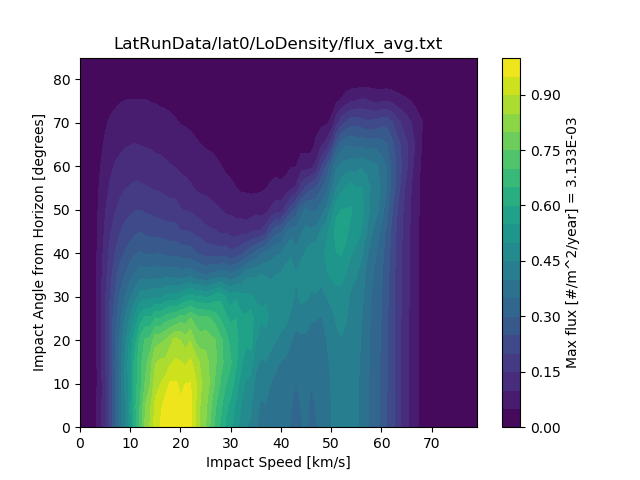
\includegraphics[width=.85\linewidth]{../LoDensity018_lat0.png}  
		\caption{Low density population impacting at the equator.}
		\label{fig:sub-LoDensity018_lat0}
	\end{subfigure}
	\begin{subfigure}{.47\textwidth}
		\centering
		% include second image
		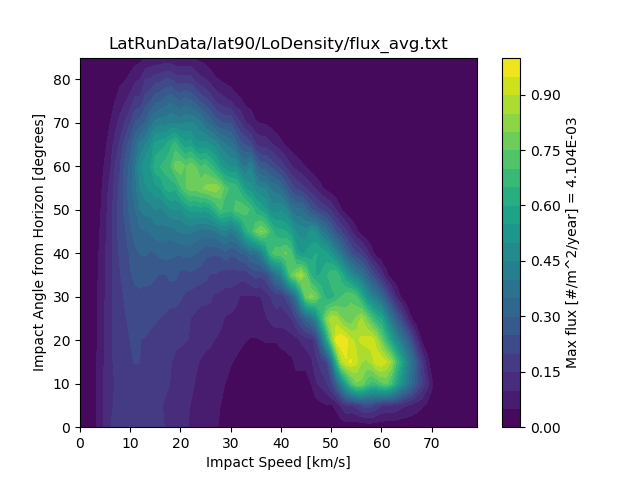
\includegraphics[width=.85\linewidth]{../LoDensity036_lat90.png}  
		\caption{Low density population impacting at the north pole.}
		\label{fig:sub-LoDensity036_lat90}
	\end{subfigure}
	\newline
	\begin{subfigure}{.47\textwidth}
		\centering
		% include third image
		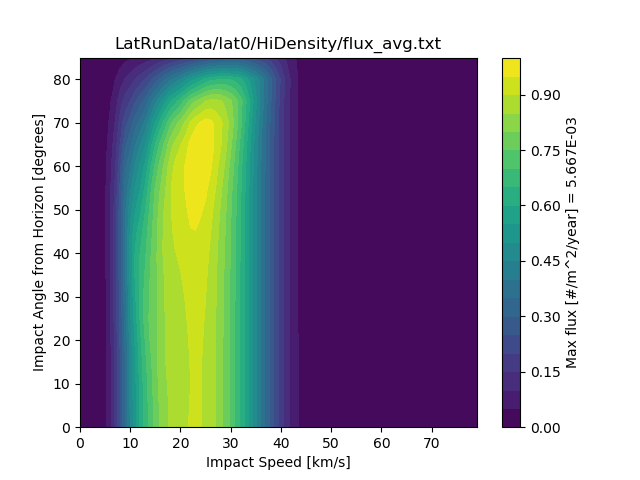
\includegraphics[width=.85\linewidth]{../HiDensity018_lat0.png}  
		\caption{High density population impacting at the equator.}
		\label{fig:sub-HiDensity018_lat0}
	\end{subfigure}
	\begin{subfigure}{.47\textwidth}
		\centering
		% include fourth image
		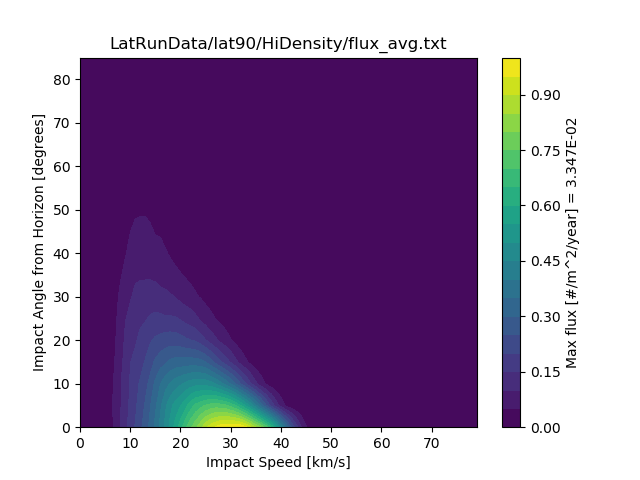
\includegraphics[width=.85\linewidth]{../HiDensity036_lat90.png}  
		\caption{High density population impacting at the north pole.}
		\label{fig:sub-HiDensity036_lat90}
	\end{subfigure}
	\caption{Fluxes (as a function of impact speed and angle from the horizon) of the low density population (a) and (b), and the high density population (c) and (d) impacting the Moon at the equator (a) and (c), and the north/south pole (b) and (d).}
	\label{fig:latitudinal_dependence}
\end{figure}

As an example, in Figure \ref{fig:latitudinal_dependence}, we show the speed-angle flux distribution at the equator and poles for the low and high density MEM populations. Note that the fluxes in the northern and southern hemispheres are symmetric about the equator. We can see from Figure \ref{fig:latitudinal_dependence} that the impact angles and speeds are highly dependent on the impact latitude on the Moon and hence warrant a more sophisticated approach to computing the secondary fluxes. We cannot assume that most impacts are at 45 degrees or are not highly oblique. How this latitude dependence affects the secondary flux is not entirely clear, except for the fact that we hypothesize that the secondary fluxes will be themselves dependent on latitude.
 
%%%%%%%%%%%%%%%%%%%%%%%%%%%%%%%%%%%%%%%%%%%%%%%%%%%%%%%%%%%%%%%%%%
%%%%%%%%%%%%%%%%%%%%%%%%%%%%%%%%%%%%%%%%%%%%%%%%%%%%%%%%%%%%%%%%%%
\subsubsection{Density Distribution Function}


The meteoroid density has two components, a low and a high density contribution, as shown in Figure \ref{fig:MEM_UG_Fig2.5_density-distribution}. To take into account this particular distribution in computing the particle flux mass spectrum, we should integrate Figure \ref{fig:MEM_UG_Fig2.5_density-distribution} against Eq.\ \ref{eq:HH11_mass-ejected1}. Since the meteoroid density components can be written in terms of log-normal distributions
\begin{equation}\label{eq:log-normal_distribution}
F_\delta(x) = \frac{A}{\sigma\sqrt{2\pi}x}\exp\left[-\frac{(\ln x-\mu_\delta)^2}{2\sigma^2}\right],
\end{equation}
the integration entails computing the moments of a log-normal distribution. The $\alpha$-~moment is given by
\begin{equation}
F^\alpha_\delta(A,\mu_\delta,\sigma) = A\exp\left(\alpha\mu_\delta+\frac{1}{2}\alpha^2\sigma^2\right).
\end{equation}
Inserting these results into Eq.\ \ref{eq:HH11_mass-ejected1}, the functional form of the projectile density contribution can be written as
\begin{equation}
F_\delta = F^{3\nu-1}_\delta(A_{low}, \mu_{low},\sigma_{low}) + F^{3\nu-1}_\delta(A_{high}, \mu_{high},\sigma_{high}),
\end{equation}
where the fit parameters for the low and high density components are shown in Figures~\ref{fig:Fit-to-MEM_low_dens} and \ref{fig:Fit-to-MEM_high_dens}. The MEM User Guide also gives these values, but assumes log-base 10 instead of log-based $e$ as we did here. %Since the meteoroid density is given in units of \textit{fraction per 50 kg m$^{-3}$}, we need to divide the $A$ constants by 50 in order to give correct units.

\begin{figure}[h!]
	\centering
	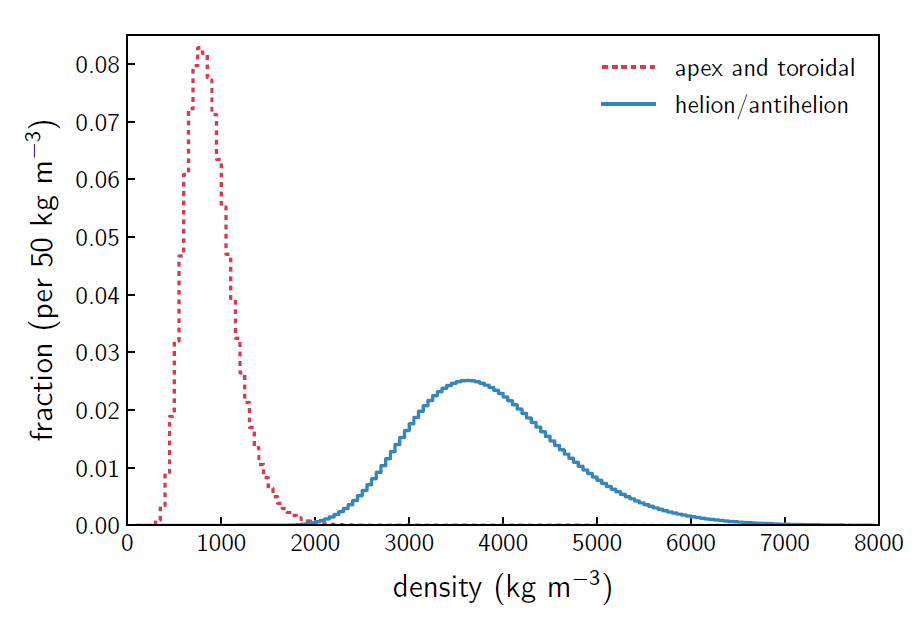
\includegraphics[scale=0.5]{../LaTeX_Report/MEM_UG_Fig2.5_density-distribution.PNG}
	\caption{Meteoroid density distribution according to the MEM3 User Guide. The apex and toroidal meteoroid sources constitute the low-density population, while the helion/antihelion source constitutes the high-density population. Each set of densities follows a log-normal distribution \citep[c.f. Figure 11,][]{moorhead2019nasa}.}\label{fig:MEM_UG_Fig2.5_density-distribution}
\end{figure}


\begin{figure}[h!]
	\centering
	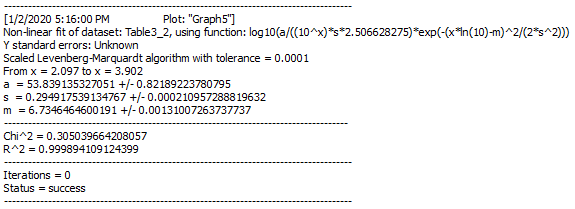
\includegraphics[scale=0.8]{../LaTeX_Report/Fit-to-MEM_low_dens.PNG}
	\caption{Non-linear fit of the low density profile in Figure \ref{fig:MEM_UG_Fig2.5_density-distribution} with Eq.\ \ref{eq:log-normal_distribution} in \textsf{SciDAVis}, giving the constants for $a\rightarrow A$, $s\rightarrow \sigma$, and $m\rightarrow \mu_\delta$.}\label{fig:Fit-to-MEM_low_dens}
\end{figure}

\begin{figure}[h!]
	\centering
	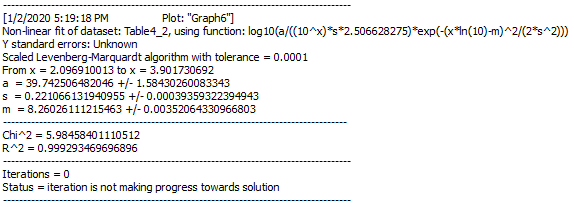
\includegraphics[scale=0.8]{../LaTeX_Report/Fit-to-MEM_high_dens.PNG}
	\caption{Non-linear fit of the high density profile in Figure \ref{fig:MEM_UG_Fig2.5_density-distribution} with Eq.\ \ref{eq:log-normal_distribution} in \textsf{SciDAVis}, giving the constants for $a\rightarrow A$, $s\rightarrow \sigma$, and $m\rightarrow \mu_\delta$.}\label{fig:Fit-to-MEM_high_dens}
\end{figure}

%%%%%%%%%%%%%%%%%%%%%%%%%%%%%%%%%%%%%%%%%%%%%%%%%%%%%%%%%%%%%%%%%%
%%%%%%%%%%%%%%%%%%%%%%%%%%%%%%%%%%%%%%%%%%%%%%%%%%%%%%%%%%%%%%%%%%
\subsubsection{Mass Spectrum}

From the MEM3 User Guide , we get the $g(m)$ flux of meteoroids larger than a limiting mass $m$, originally from \cite{grun1985collisional}. The Gr{\"u}n interplanetary flux equation is given by
\begin{equation}\label{eq:Grun_flux}
g(m) = (c_4m^{\gamma_4}+c_5)^{\gamma_5} + c_6(m + c_7m^{\gamma_6} + c_8m^{\gamma_7})^{\gamma_8} + c_9(m + c_{10}m^{\gamma_9})^{\gamma_{10}},
\end{equation}
where the constants are $c_4 = 2.2\times 10^3$, $c_5 = 15$, $c_6 = 1.3 \times 10^{-9}$, $c_7=10^{11}$, $c_8=10^{27}$, $c_9 = 1.3\times 10^{-16}$, $c_{10} = 10^6$; and the exponents are $\gamma_4 = 0.306$, $\gamma_5 = -4.38$, $\gamma_6 = 2$, $\gamma_7 = 4$, $\gamma_8 = -0.36$, $\gamma_{9} = 2$, and $\gamma_{10} = -0.85$. Eq.\ \ref{eq:Grun_flux} is applied to MEM's mass range and is shown in Figure \ref{fig:MEM_UG_Fig2.1_partile-mass-distribution}.

\begin{figure}[h!]
	\centering
	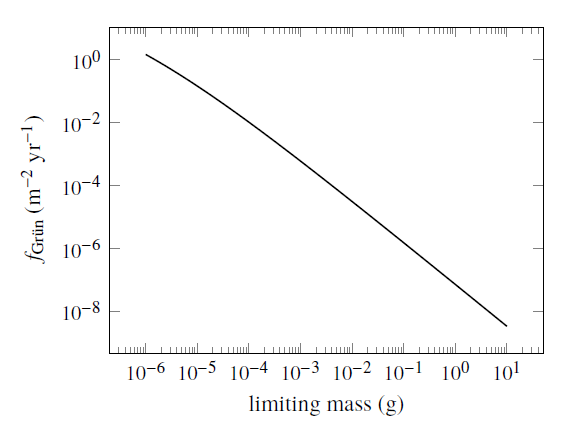
\includegraphics[scale=0.65]{../LaTeX_Report/MEM_UG_Fig2.1_partile-mass-distribution.PNG}
	\caption{The Gr{\"u}n interplanetary meteoroid flux as a function of limiting particle mass \citep[Figure 1]{moorhead2019nasa}.}\label{fig:MEM_UG_Fig2.1_partile-mass-distribution}
\end{figure}

The mass flux $dg(m)/dm$ and Eq.\ \ref{eq:HH11_mass-ejected1} should be integrated over the mass range $m_{min} = 10^{-6}$ g to $m_{max} = 10^1$~g in order to account for all impactor mass sizes, which we call $G_m$ given as
\begin{equation}\label{eq:Gm_integral}
G_m = \int_{m_{min}}^{m_{max}}dm\frac{-dg(m)}{dm}m.
\end{equation}

The mass flux $dg(m)/dm$ can be fit to a double power law
\begin{equation}\label{eq:Grun_mass_flux}
\frac{dg(x)}{dx} = \frac{1}{ax^b+cx^d},
\end{equation}
where the fit parameters are shown in Figure \ref{fig:Fit-to-D_Grun}, using a log-log scale to capture the small and large masses correctly.

\begin{figure}[h!]
	\centering
	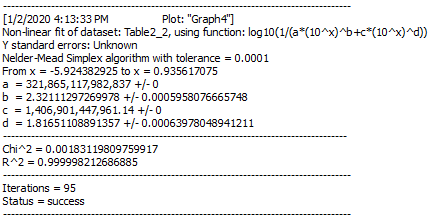
\includegraphics[scale=1]{../LaTeX_Report/Fit-to-D_Grun.PNG}
	\caption{Non-linear fit of Figure \ref{fig:MEM_UG_Fig2.1_partile-mass-distribution} with Eq.\ \ref{eq:Grun_mass_flux} in \textsf{SciDAVis}, giving the constants for $a$, $b$, $c$, and $d$.}\label{fig:Fit-to-D_Grun}
\end{figure}

%%%%%%%%%%%%%%%%%%%%%%%%%%%%%%%%%%%%%%%%%%%%%%%%%%%%%%%%%%%%%%%%%%
%%%%%%%%%%%%%%%%%%%%%%%%%%%%%%%%%%%%%%%%%%%%%%%%%%%%%%%%%%%%%%%%%%
\subsection{Near-Earth Object Environment}\label{ssec:NEO}

The near-Earth object (NEO) environment introduces mass sizes of impactors beyond 10 g, outside of MEM's size range. Unlike MEM, the NEO's consist of small asteroids and comets between 0.1 and 1000 m in diameter. The work outlined in this section originates from analysis done by Althea Moorhead (see Memo OSMA/MEO/Lunar-001). The goal of the this analysis converts energy-limited fluxes of NEO's at the Earth to mass-limited fluxes at the Moon using \cite{brown2002flux} as a starting point.

%%%%%%%%%%%%%%%%%%%%%%%%%%%%%%%%%%%%%%%%%%%%%%%%%%%%%%%%%%%%%%%%%%
%%%%%%%%%%%%%%%%%%%%%%%%%%%%%%%%%%%%%%%%%%%%%%%%%%%%%%%%%%%%%%%%%%
\subsubsection{Kinetic-Energy-Limited Flux}

\cite{brown2002flux} use a combination of bright bolide data, infrared and acoustic data, satellite observations, and telescopic observations of small asteroids to construct a power law describing the cumulative flux of large objects onto Earth, given by
\begin{equation}
\log_{10}N = a-b\log_{10}\text{KE},
\end{equation}
where KE is the kinetic energy of the impactor in kilotons TNT equivalent ($4.184\times 10^{12}$ J), N is the number of objects impacting the Earth per year with a given kinetic energy or greater, and the constants are $a = 0.5677$ and $b=0.9$.

We convert this flux to MKS units by assuming the Earth has an effective radius of 6471 km (including 100 km of atmosphere capable of ablating meteoroids). The resulting kinetic-energy-limited flux per square meter per year is given by
\begin{equation}\label{eq:NEO_KE_flux}
f_\Earth(\text{KE}) = 7.023\times 10^{-15} \text{KE}^{-0.9}.
\end{equation}
To obtain Equation \eqref{eq:NEO_KE_flux}, we have divided by the surface are of the Earth. Thus, $f_\Earth$ reports the flux per unit surface area. One can convert Equation \eqref{eq:NEO_KE_flux} to a flux per cross-sectional are, if desired, by multiplying by 4. Note that the bulk density is assumed to be 3000 kg m$^{-3}$ \citep{brown2002flux}.

%%%%%%%%%%%%%%%%%%%%%%%%%%%%%%%%%%%%%%%%%%%%%%%%%%%%%%%%%%%%%%%%%%
%%%%%%%%%%%%%%%%%%%%%%%%%%%%%%%%%%%%%%%%%%%%%%%%%%%%%%%%%%%%%%%%%%
\subsubsection{Mass-Limited Flux}

The mass-limited flux at the lunar surface can be shown to be
\begin{equation}\label{eq:NEO_mass_factor_int}
g_\leftmoon (m) = 2.89\times 10^{-11} \text{m}^{-2}\text{yr}^{-1}\cdot m^{-0.9},
\end{equation}
where $m$ is the mass of the impactor in kg.

When converting the NEO flux into secondary flux using Equation \eqref{eq:HH11_mass-ejected1}, we must integrate the flux per mass with $m$
\begin{equation}
G_{\leftmoon m} = \int_{m_{min}}^{m_{max}}dm\frac{-d g_\leftmoon(m)}{dm}m,
\end{equation}
where 
\begin{equation}
\frac{d g_\leftmoon(m)}{dm} = -2.601 \times 10^{-11} \text{m}^{-2}\text{yr}^{-1}\cdot m^{-1.9}.
\end{equation}

Therefore, using $m_{min} = 10 $ g (extrapolating down to the upper-limit of MEM) and $m_{max} = 1.57 \times 10^{15}$ g (mass of a sphere taking 1000 m as the diameter and 3000 kg m$^{-3}$ as the density), Equation \eqref{eq:NEO_mass_factor_int} becomes
\begin{equation}
G_{\leftmoon m} = 4.148 \times 10^{-9} \text{m}^{-2}\text{yr}^{-1} \cdot \text{kg},
\end{equation}
which represents the mass flux in the given range above.

%%%%%%%%%%%%%%%%%%%%%%%%%%%%%%%%%%%%%%%%%%%%%%%%%%%%%%%%%%%%%%%%%%
%%%%%%%%%%%%%%%%%%%%%%%%%%%%%%%%%%%%%%%%%%%%%%%%%%%%%%%%%%%%%%%%%%
\subsubsection{Speed Distribution}
The speed distribution of NEO's is shown in Figure \ref{fig:vmass}. The values (fraction of flux per bin) in each bin are midpoint values, where the bins have a size of 2 km s$^{-1}$. Note also that because the flux is a power law, this speed distribution is independent of limiting mass.

\begin{figure}[h!]
	\centering
	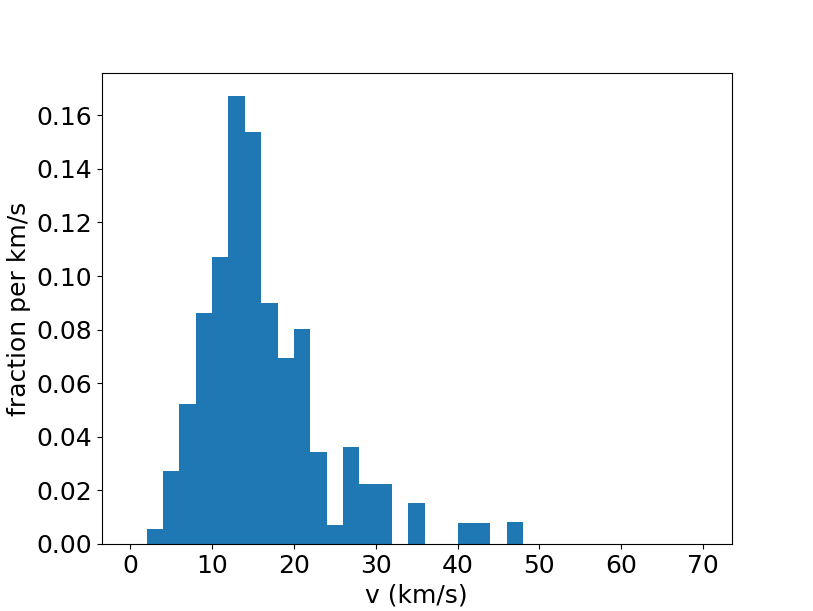
\includegraphics[scale=0.50]{../NEA_Brown/vmass.png}
	\caption{Mass-limited speed distribution at the lunar surface.}\label{fig:vmass}
\end{figure}


%%%%%%%%%%%%%%%%%%%%%%%%%%%%%%%%%%%%%%%%%%%%%%%%%%%%%%%%%%%%%%%%%%
%%%%%%%%%%%%%%%%%%%%%%%%%%%%%%%%%%%%%%%%%%%%%%%%%%%%%%%%%%%%%%%%%%
\section{Output Environment Format}\label{sec:outputEnv}

The output format is based on the igloo file type of MEM, see Figure \ref{fig:example_igloo} for an example.

\begin{figure}[h!]
	\centering
	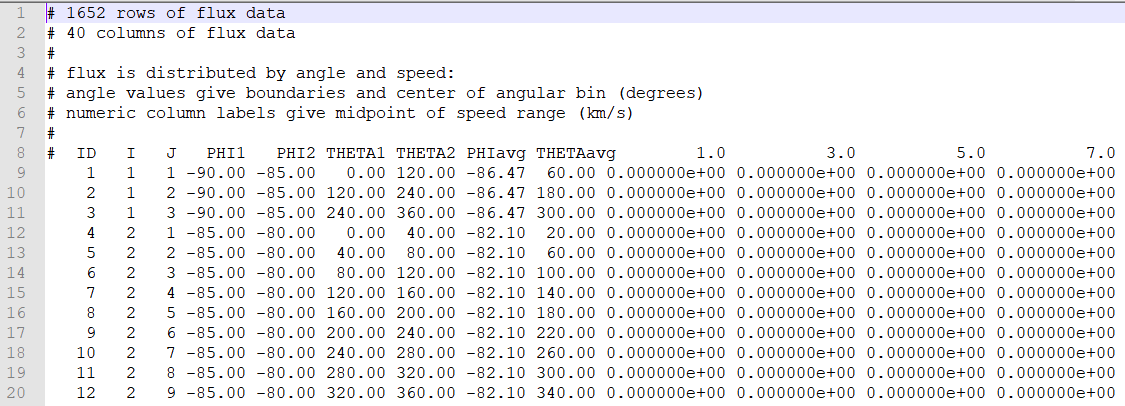
\includegraphics[scale=0.50]{../LaTeX_Report/example_igloo.png}
	\caption{Example of the igloo file format from MEM.}\label{fig:example_igloo}
\end{figure}

The igloo format attempts to give solid-angle bins of roughly equal size throughout the whole spherical grid. If a normal division of altitude and azimuth was used, the poles would be highly sampled and would have proportionally smaller solid-angle bin sizes compared with the equatorial region. See the MEM User Guide \citep{moorhead2019nasa} for more details.



%%%%%%%%%%%%%%%%%%%%%%%%%%%%%%%%%%%%%%%%%%%%%%%%%%%%%%%%%%%%%%%%%%
%%%%%%%%%%%%%%%%%%%%%%%%%%%%%%%%%%%%%%%%%%%%%%%%%%%%%%%%%%%%%%%%%%
\subsection{Mass Limited Speed-Solid Angle Flux Distribution}

Just like in the MEM, we provide the mass limited speed-solid angle flux distribution, but for the secondary flux. We can compute the secondary flux for any location on the Moon. The flux distribution is in units of number per square meter per year in bins of speed, azimuth, and altitude. We chose speed bins of 100 m s$^{-1}$ to 250~m~s$^{-1}$, 250 m s$^{-1}$ to 1000 m s$^{-1}$, and 1000 m s$^{-1}$ to 2400 m s$^{-1}$ (i.e., the escape speed of the Moon). The altitude is divided into 10 degree bins while the azimuth\footnote{East is 0 degrees and the azimuth increases in a counter-clockwise fashion.} is divided into 20 degree bins.

%%%%%%%%%%%%%%%%%%%%%%%%%%%%%%%%%%%%%%%%%%%%%%%%%%%%%%%%%%%%%%%%%%
%%%%%%%%%%%%%%%%%%%%%%%%%%%%%%%%%%%%%%%%%%%%%%%%%%%%%%%%%%%%%%%%%%
\newpage
\section{Secondary Ejecta Model}\label{sec:ejectaModel}

%%%%%%%%%%%%%%%%%%%%%%%%%%%%%%%%%%%%%%%%%%%%%%%%%%%%%%%%%%%%%%%%%%
%%%%%%%%%%%%%%%%%%%%%%%%%%%%%%%%%%%%%%%%%%%%%%%%%%%%%%%%%%%%%%%%%%
\subsection{Assumptions and Simplifications}\label{ssec:assumptions}

There are several assumptions and simplications made in our model in order to provide traceable engineering solutions. We provide a list below with the most important assumptions in no particular order and provide comments on each.
\begin{enumerate}
	\item The ejecta particle distribution is the same as the virgin regolith particle distribution.
	\begin{itemize}
		\item Crater sizes that are less than $\sim50$ m will mostly sample the top-most layer of regolith. For impactors that generate larger craters, such as those found in the NEO population, this assumption breaks down. We expect the very large craters ($> 100$ m) to introduce larger bolder sizes not present in the virgin regolith particle distribution. We believe these large bolders to be in the far tail of the distribution function and are very unlikely. Ignoring the large particle population will inflate the smaller particle sizes, which may help to offset the error in the risk, but this offset is not for certain.
	\end{itemize}
	\item The scaling law provided by \cite{housen2011ejecta} is valid for all impactors simulated in our model.
	\begin{itemize}
		\item Both authors are experts in the field of high-velocity impacts and have done much work to develop scaling laws that are valid for several orders of magnitude of impact sizes. For extremely small size impacts, such as impactor masses near $10^{-6}$ g, the scaling laws might not be valid since this is roughly the 50-percentile size of the regolith particle size distribution. For simplification, we ignore this issue for now. 
	\end{itemize}
	\item The azimuth and zenith angle distribution functions are given empirically and do not depend on the size of impact or speed of impact, only the angle of impact.
	\begin{itemize}
		\item The azimuth distribution function follows published work done by ESA contract work \citep{ESABASE2_DebrisRelease10.0}. We modified the azimuth distribution function at highly oblique angles to include information about ejecta patterns that exhibit the so called butterfly pattern \citep{shuvalov2011ejecta}. Depending on the latitude of the impact location, there can be a substantial component of the flux that can come into play.
		\item The zenith angle distribution does have an azimuthal and impact angle dependence that follows fits from \cite{gault1978experimental}. When the outgoing zenith angle tips over (when it goes negative), we ignore this component as an exclusion zone and implicitly include the fluxes in the downstream direction. This avoids having to deal with multi-valued functions which would require special cases to handle.
		\item Since the integration is complicated enough, we do not want to complicate things by introducing a velocity dependence in the angle distributions. We know this to be the case in reality, but we ignore this dependence for simplicity.
	\end{itemize}
	\item The regolith density is constant over the whole Moon and for all depths.
	\begin{itemize}
		\item The regolith density differs from highlands to mare in addition to depth. However, building a density map of the Moon is beyond the scope of this engineering model. We also note that the density dependence is raised to a small power ($\sim 0.2$), so this will have a minor effect on total mass ejected from the crater. On the other hand, density can have a great impact on ballistic equations and bumper computations.
	\end{itemize}
	\item The Moon is a perfect sphere with a mono-polar gravity well (i.e., we ignore irregularities in the lunar surface and gravity).
	\begin{itemize}
		\item We expect landing locations to not be deep in craters, which can be hazardous to con-ops. Local terrain can have a shadowing effect, so our calculations could be seen as a worst-case in this sense since we ignore these.
		\item Most of the ejecta will have relatively short transit times and therefore will only be slightly perturbed by the irregular gravity well of the Moon. We also ignore Coriolis forces, which can be shown to be insignificant on the Moon for all relevant ejecta speeds.
	\end{itemize}
	\item The angular distribution of NEA's on the lunar surface are modeled after the high density population provided by MEM.
	\begin{itemize}
		\item Roughly speaking, the NEA's we consider are in the ecliptic plane, as is the high density population of sporadic meteors in MEM. The speed distributions do differ so we re-scale the angular distribution from MEM using the NEA speed distribution.
	\end{itemize}
\end{enumerate}


%%%%%%%%%%%%%%%%%%%%%%%%%%%%%%%%%%%%%%%%%%%%%%%%%%%%%%%%%%%%%%%%%%
%%%%%%%%%%%%%%%%%%%%%%%%%%%%%%%%%%%%%%%%%%%%%%%%%%%%%%%%%%%%%%%%%%
\subsection{Conversion from Primary to Secondary Flux}

The total mass flux of secondary ejecta can be found from properties of the primary impactor. From \cite{housen2011ejecta}, we can compute the mass ejected faster than $v$ in terms of impactor properties, given by
\begin{eqnarray}\label{eq:HH11_mass-ejected1}
M(v; \rho; m, \delta, U, \alpha) = M(>v) = C_4 m\left[\frac{v}{U\Theta(\alpha)}\left(\frac{\rho}{\delta}\right)^{\frac{3\nu-1}{3\mu}}\right]^{-3\mu},
\end{eqnarray}
where
\begin{itemize}
	\item $v$: secondary ejecta speed,
	\item $\rho$: target density,
	\item $m$: projectile mass,
	\item $\delta$: projectile density,
	\item $U$: projectile speed,
	\item $\alpha$: projectile impact angle (from horizon),
\end{itemize}
and
\begin{eqnarray}
C_4 = \frac{3k}{4\pi}C_1^{3\mu},
\end{eqnarray}
where the constants $k$, $C_1$, $\nu$, and $\mu$ depend on the specific material properties, see Table 3 of \cite{housen2011ejecta}. The impact angle modification equation $\Theta(\alpha)$ can be chosen to be
\begin{equation}
\Theta(\alpha) = \begin{cases}
1\\
\sin\alpha\\
\sin^\eta\alpha
\end{cases},
\end{equation}
where typical values of $\eta$ lie between 1 and 2. For the ejected mass that is in a given velocity range, we can define $\Delta M(v_2, v_1)$ as
\begin{equation}\label{eq:delta_M}
\Delta M(v_2, v_1) = M(>v_2) - M(>v_1).
\end{equation}

Equation \eqref{eq:HH11_mass-ejected1} only gives us the total mass ejecta from the impact. We need to know what portion of that total mass reaches a particular region of interest. In essence, this is the major effort of the model outlined in this report. In the following section, we will show how to compute the portion of total mass.

%%%%%%%%%%%%%%%%%%%%%%%%%%%%%%%%%%%%%%%%%%%%%%%%%%%%%%%%%%%%%%%%%%
%%%%%%%%%%%%%%%%%%%%%%%%%%%%%%%%%%%%%%%%%%%%%%%%%%%%%%%%%%%%%%%%%%
\subsection{Secondary Ejecta Distribution Function}


The mass ejected from the crater, $M(>v)$, from Eq.\ \eqref{eq:HH11_mass-ejected1}, is the total mass ejected from an impact at velocities greater than $v$. However, we would like to know how this ejecta is distributed in speed and solid angle so we can map the ejecta to a particular surface location on the Moon. We can then set Eq.\ \eqref{eq:HH11_mass-ejected1} in terms of the integral over the distribution functions of speed and solid angle as
\begin{equation}
M(>v) = \int_{v}^{\infty}\int_{0}^{2\pi}\int_{0}^{\pi/2}\sin\alpha d\alpha d\beta dv' F(\alpha)G(\beta)H(v'),
\end{equation} 
where $\alpha$ is the zenith angle, $\beta$ is the azimuth angle, and $v$ is the ejecta speed. Just to note, at the secondary impact location, the zenith angle will be the same as the ejected zenith angle. However, the azimuth angle (or bearing) will be modified due to travel across a spherical surface, see Section \ref{ssec:Distance_and_Bearing}.

%%%%%%%%%%%%%%%%%%%%%%%%%%%%%%%%%%%%%%%%%%%%%%%%%%%%%%%%%%%%%%%%%%
%%%%%%%%%%%%%%%%%%%%%%%%%%%%%%%%%%%%%%%%%%%%%%%%%%%%%%%%%%%%%%%%%%
\subsubsection{Speed Distribution Function}


The speed distribution $H(v')$ is defined by
\begin{equation}
\int_{v}^{\infty}dv'H(v') = v^{-3\mu},
\end{equation}
which is the speed dependent term of Eq.\ \eqref{eq:HH11_mass-ejected1}. We can then solve the speed distribution explicitly as
\begin{equation}
H(v) = 3\mu v^{-(3\mu+1)}.
\end{equation}

To integrate over the velocity distribution, we must take the results from Section~\ref{sssec:ZenithDistributionFunction} on the zenith distribution function and combine them with the above integral, giving

\begin{align}
&3\mu\int_{v_0}^{v_1}dv v^{-(3\mu+1)}\Delta x(v)\left[1-\frac{x_0(v)+x_1(v)}{2}\right]^a \left[\frac{x_0(v)+x_1(v)}{2}\right]^{1/a}\\
=& 3\mu\int_{v_0}^{v_1}dv v^{-(3\mu+1)}(\Delta m v + \Delta b)(1-m_{avg}v-b_{avg})^a(m_{avg}v + b_{avg})^{1/a}\\
=& \int_{v_0}^{v_1}dv H_2(v),\label{eq:def_H2}
\end{align}
where
\begin{align}
\Delta m & = m_1 - m_0,\\
\Delta b &= b_1 - b_0,\\
m_{avg} &= \frac{m_0+m_1}{2},\\
b_{avg} &= \frac{b_0+b_1}{2}.
\end{align}

This integral is related to the Appell F1 multivariate hypergeometric function and cannot be simplified to a finite number of single variable hypergeometric functions for generalized values of the exponent $a$. At this time, we will defer to integrate this equation numerically, preferably using the Romberg integration method.

Alternatively, we can attempt to generate an approximation. Taking the Taylor expansion of Equation \eqref{eq:def_H2} about $v_{avg}$ out to the first term, we have (note, the first term drops out of the integral during integration, so the error is of order $\Delta v^3$)
\begin{align}
\int_{v_0}^{v_1}dv H_2(v) &\sim \int_{v_0}^{v_1}dv[H_2(v_{avg}) + H_2'(v_{avg})(v-v_{avg})+\dots],\\
&= \Delta v H_2(v_{avg}),\nonumber
\end{align}
\begin{equation}
=3\mu\Delta v v_{avg}^{-(3\mu+1)}(\Delta m v_{avg} + \Delta b)(1-m_{avg}v_{avg}-b_{avg})^a(m_{avg}v_{avg} + b_{avg})^{1/a},
\end{equation}
where
\begin{align}
\Delta v &= v_1-v_0,\\
v_{avg} &= \frac{v_0 + v_1}{2}.
\end{align}


%%%%%%%%%%%%%%%%%%%%%%%%%%%%%%%%%%%%%%%%%%%%%%%%%%%%%%%%%%%%%%%%%%
%%%%%%%%%%%%%%%%%%%%%%%%%%%%%%%%%%%%%%%%%%%%%%%%%%%%%%%%%%%%%%%%%%
\subsubsection{Zenith Angle Distribution Function}\label{sssec:ZenithDistributionFunction}

To complete the integral over the zenith distribution, namely
\begin{equation}\label{eq:zenith_integral}
\int_{\alpha_0(v)}^{\alpha_1(v)}d\alpha\sin\alpha F(\alpha),
\end{equation}
we need to choose a distribution function for $F(\alpha)$ to allow for analytic solutions. We will therefore look for an alternate distribution given by the form
\begin{equation}
F(\alpha) = (1-\cos\alpha)^{1/a}\cos^a\alpha,
\end{equation}
where the exponent $a$ can be defined in terms of the peak angle $\alpha_{max}$ as
\begin{equation}\label{eq:a_exponent}
a = \frac{\cos\alpha_{max}}{1-\cos\alpha_{max}} = \frac{\cos\alpha_{max}}{2\sin^2(\alpha_{max}/2)},
\end{equation}
such that $F'(\alpha_{max}) = 0$ and $F''(\alpha_{max}) < 0$.

In order to compare with experiments for the peak angle $\alpha_{max}$, we can use Figure~18 of \cite{gault1978experimental} as a proxy to our model of $\alpha_{max}$, as a function of the azimuth angle. Using a third order polynomial for both fits to the downstream and upstream angles given in Table \ref{tab:upstream_downstream_angles}, we arrive at
\begin{align}
\alpha_{max}(\beta - \beta_i = \pi) &= 0.0003\alpha_i^3 - 0.036\alpha_i^2 + 1.5206\alpha_i + 20, \text{ downstream}\\
\alpha_{max}(\beta - \beta_i = 0) &= -0.00042\alpha_i^3 + 0.0236\alpha_i^2 + 0.129\alpha_i + 20, \text{ upstream}
\end{align}
in units of degrees, where $\beta_i$ is the impact azimuth angle, $\beta$ is the ejecta azimuth angle, and $\alpha_i$ is the impact zenith angle. For other values of $\beta - \beta_i$, we can write a complete function as
\begin{equation}
\alpha_{max}(\beta) = \alpha_{max}(\beta - \beta_i = \pi)\cdot \sin^2\left(\frac{\beta - \beta_i}{2}\right)
+ \alpha_{max}(\beta - \beta_i = 0)\cdot \cos^2\left(\frac{\beta - \beta_i}{2}\right),
\end{equation}
or rewriting we have
\begin{equation}
\alpha_{max}(\beta) = \frac{\alpha_{max,0}+\alpha_{max,\pi}}{2} - \frac{\alpha_{max,\pi}-\alpha_{max,0}}{2}\cos(\beta-\beta_i),
\end{equation}
and solving for $\beta-\beta_i$, after setting $\alpha_{max}(\beta)$ to zero,
\begin{equation}
\arccos\left(\frac{\alpha_{max,0}+\alpha_{max,\pi}}{\alpha_{max,\pi}-\alpha_{max,0}}\right) = \beta-\beta_i.
\end{equation}
As a simplification, we can approximate the $\cos(\beta-\beta_i)$ term as (note, this is not a Taylor series)
\begin{equation}
\cos(\beta-\beta_i) \sim 1 - \left|\frac{\beta-\beta_i}{\pi/2}\right|,
\end{equation}
for $-\pi \le \beta-\beta_i \le \pi$ such that $\cos\alpha_{max}$ becomes
\begin{equation}\label{eq:cos_a_max_approx}
\cos\alpha_{max} \sim \cos\left[\alpha_{max,0}+\frac{\alpha_{max,\pi}-\alpha_{max,0}}{\pi}|\beta-\beta_i|\right]
\end{equation}

\begin{table}[h]\centering
	\caption{Cone angles of upstream and downstream of impact derived from Figure 18 of \cite{gault1978experimental}.}\label{tab:upstream_downstream_angles}
	\begin{tabular}{|c | c | c |}\hline
		Impact Zenith Angle & Upstream Zenith Angle & Downstream Zenith Angle\\\hline
		0	&20	&20\\\hline
		15	&24	&35\\\hline
		30	&35	&45\\\hline
		45	&28	&40\\\hline
		60	&13	&54\\\hline
		75	&-35	&66\\\hline		
	\end{tabular}
\end{table}
Using Table \ref{tab:upstream_downstream_angles} as a fit for the peak angle $\alpha_{max}$ is an approximation since the tabular data is only for a specific snapshot of the ejecta at a side view, $90^\circ$ from the impact direction. The zenith distribution should also be a function of the ejecta speed, but we do not make this assumption for the sake of simplicity. According to this model, starting around $60^\circ - 70^\circ$, there is a region of exclusion for a part of the zenith distribution upstream of the impact, see Figure \ref{fig:ExlusionRange_vs_ImpactAngle}.


\begin{figure}[h!]
	\centering
	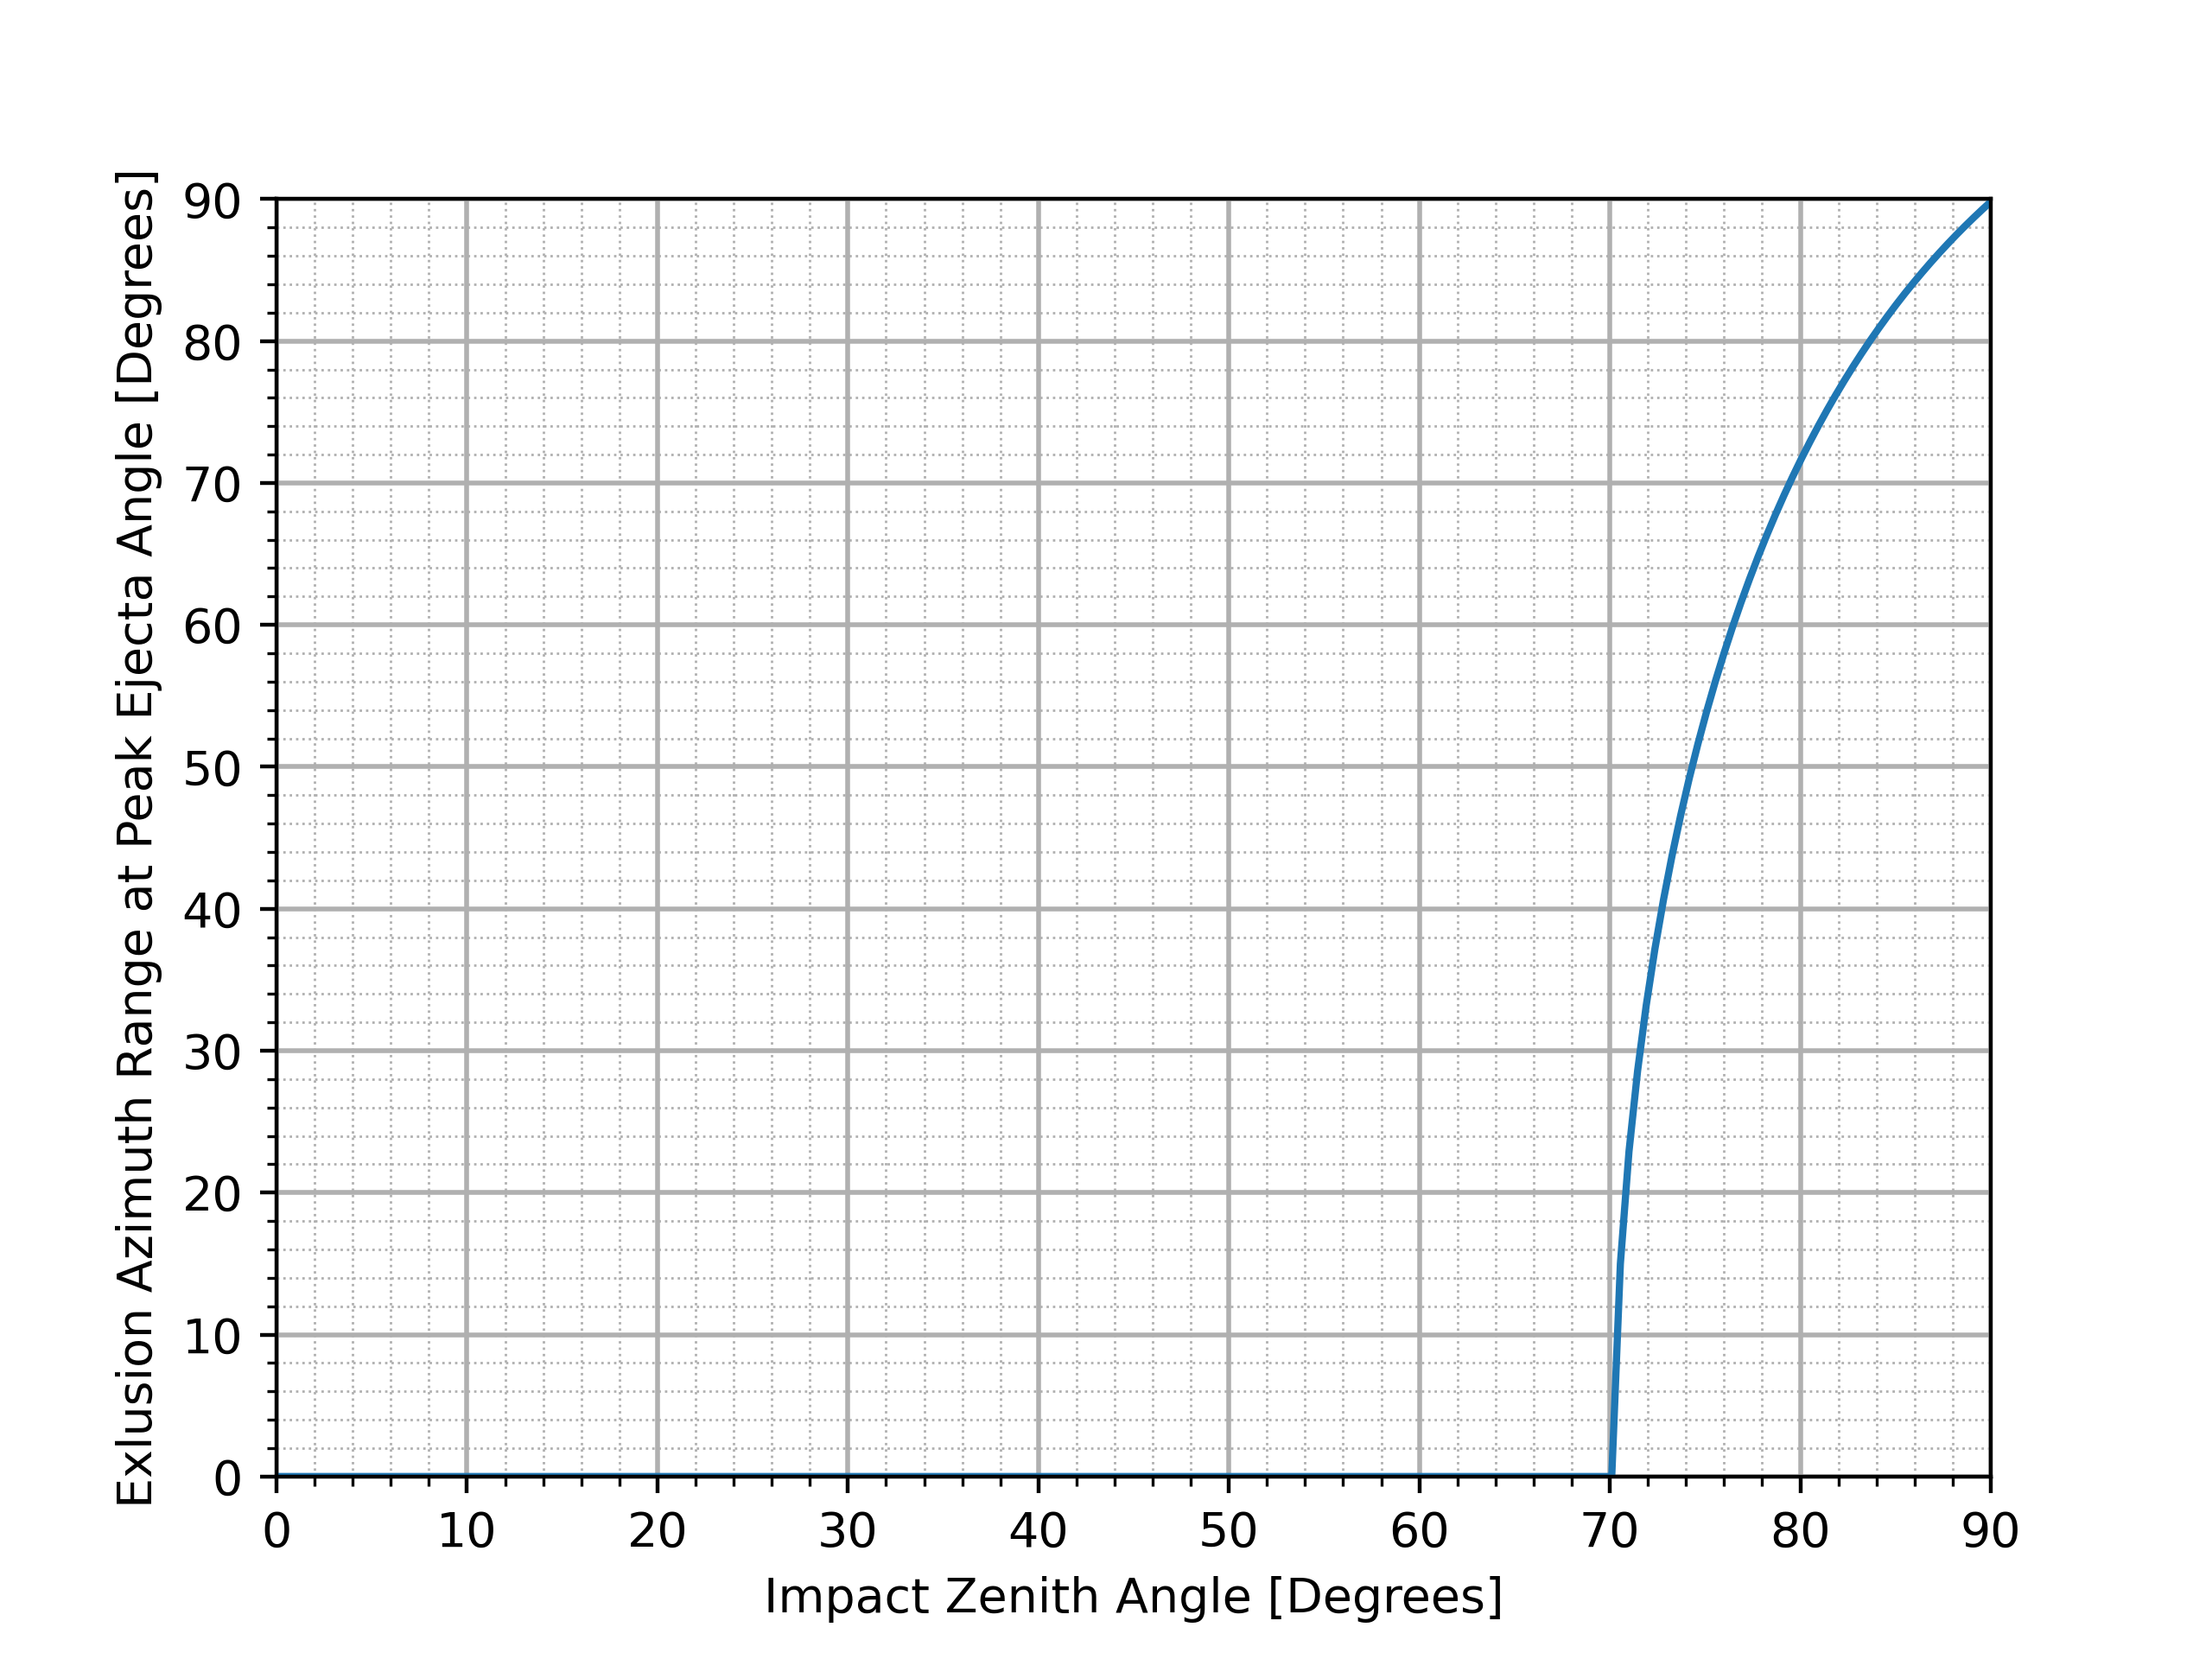
\includegraphics[scale=0.65]{../LaTeX_Report/ExlusionRange_vs_ImpactAngle.png}
	\caption{For larger impact angles that are more grazing to the surface, the zenith and azimuth ejecta distributions become asymmetric. Starting at $70^\circ$, the peak ejecta angle $\alpha_{max}$ becomes negative in an exclusion range, as shown in the figure. This means that the $-\alpha_{max}\to\alpha_{max}$ and $\beta-\beta_i\to \beta-\beta_i +\pi$. In this model, for impact angles near $90^\circ$, most of the ejecta is concentrated in the downstream direction.}\label{fig:ExlusionRange_vs_ImpactAngle}
\end{figure}

%
%\begin{tikzpicture}\centering
%\begin{axis}[
%	xlabel = Impact Zenith Angle,
%	ylabel = Exlusion Azimuth Range at Peak Ejecta Angle
%]
%\addplot coordinates {
%	( 338.1, 266.45 )
%	( 169.1, 143.43 )
%	( 84.5, 64.80 )
%	( 42.3, 34.19 )
%	( 21.1, 9.47 )
%};
%\end{axis}
%\end{tikzpicture}

Next, we can do a variable substitution (chosen so the domain of the zenith angle to the new variable goes from $\alpha\in [0,\pi/2]$ to $x\in [0,1]$)
\begin{align}
1-x &= \cos\alpha,\\
dx &= \sin\alpha d\alpha,
\end{align}
so that Eq.\ \eqref{eq:zenith_integral} becomes
\begin{equation}\label{eq:zenith_integral2}
\int_{x_0(v)}^{x_1(v)}dx x^{1/a}(1-x)^a,
\end{equation}
where the equations $x_0(v)$ and $x_1(v)$ are a linear function of $v$ and an implicit function of the distances $D_0$ and $D_1$, respectively. The integral in Eq.\ \eqref{eq:zenith_integral2} is the incomplete beta function
\begin{equation}\label{eq:zenith_integral3}
\int_{x_0(v)}^{x_1(v)}dx x^{1/a}(1-x)^a
= \beta(x_1(v); 1/a+1, a+1) - \beta(x_0(v); 1/a+1, a+1).
\end{equation}
Note that the normalization term for $\alpha\in [0, \pi/2]$ is given by
\begin{equation}
\int_{0}^{\pi/2}d\alpha\sin\alpha F(\alpha) = 
\beta(1/a+1, a+1) = \frac{\Gamma(1/a+1)\Gamma(a+1)}{\Gamma(a+1/a+2)},
\end{equation}
which includes ejecta at speeds greater than the escape speed.

For small differences in $D_0$ and $D_1$, we can roughly assume small differences\footnote{If $\Delta x$ is not small, then we can partition the $x$ range into smaller pieces so that $\Delta x$ is small, which will be the case in almost all circumstances.} in $x_0(v)$ and $x_1(v)$ so that we can write Eq.\ \eqref{eq:zenith_integral3} in terms of a derivative, where we evaluate the derivative at the midpoint
\begin{align}
&\beta(x_1(v); 1/a+1, a+1) - \beta(x_0(v); 1/a+1, a+1)\nonumber\\
= &\frac{\beta(x_0(v) +\Delta x; 1/a+1, a+1) - \beta(x_0(v); 1/a+1, a+1)}{\Delta x}\Delta x\nonumber\\
\approx & \Delta x\frac{d}{d(x_0(v))}\beta(x_0(v); 1/a+1, a+1)\Bigr|_{x_0(v)\to x_0(v) +\Delta x/2}\nonumber\\
=& \Delta x\left[1-x_0(v)\right]^a x_0^{1/a}(v)\Bigr|_{x_0(v)\to x_0(v) +\Delta x/2}\nonumber\\
=&\Delta x(v)\left[1-\frac{x_0(v)+x_1(v)}{2}\right]^a \left[\frac{x_0(v)+x_1(v)}{2}\right]^{1/a},
\end{align}
where $\Delta x(v) = x_1(v) - x_0(v)$, and (note, the $v$'s are normalized by $v_{esc}$, emitted for clarity)
\begin{align}
x_0(v) &= m_0 v + b_0,\\
x_1(v) &= m_1 v + b_1,\\
\Delta x(v) &= (m_1-m_0)v + b_1 - b_0.
\end{align}
The coefficients $m_0, m_1$ and $b_0, b_1$ are implicit functions of the distances $D_0, D_1$. For the $j-$th distance $D_j$ and the $i-$th speed $v_i$, the $m$ and $b$ coefficients can be written as
\begin{align}
m_{j,i}^{\pm} &= \frac{v_{i+1}-v_i}{x_{j,i+1}^{\pm}-x_{j,i}^{\pm}},\\
b_{j,i}^{\pm} &= v_i - m_{j,i}^{\pm}\cdot x_{j,i}^{\pm},
\end{align}
where
%\begin{align}
%x_{j,i}^{\pm} &= 1 - \cos\alpha_{j,i}^{\pm}, \\
%\cos\alpha_{j,i}^{\pm} &= \frac{\cot\alpha_{j,i}^{\pm}}{\sqrt{1+ \cot^2\alpha_{j,i}^{\pm}}},
%\end{align}
%for (using Eq.\ \eqref{eq:gammaVs_V_D})
%\begin{equation}
%\cot\alpha_{j,i}^{\pm} = v_i^2\cot\left(\frac{D_j}{2r_m}\right) \pm \sqrt{v_i^4\cot^2\left(\frac{D_j}{2r_m}\right) +2v_i^2-1 }.
%\end{equation}

\begin{equation}
x_{j,i}^{\pm} = 1 - \cos\alpha_{j,i}^{\pm},
\end{equation}
for
\begin{equation}
\cos^2\alpha_{j,i}^{\pm} = \frac{v_i^2+\tan^2\left(\frac{D_j}{2r_m}\right)(2v_i^2-1) \pm \sqrt{v_i^4 + \tan^2\left(\frac{D_j}{2r_m}\right)(2v_i^2-1)}}{2v_i^2\left(1 + \tan^2\left(\frac{D_j}{2r_m}\right)\right) },
\end{equation}
taking the positive root, $\cos\alpha_{j,i}^{\pm} = +\sqrt{\cos^2\alpha_{j,i}^{\pm}}$, since $\alpha\in [0, \pi/2]$. Other useful transformed equations are
\begin{equation}
\tan\left(\frac{D_j}{2r_m}\right) = \frac{2v_i^2(1-x_{j,i}^{\pm})\sqrt{x_{j,i}^{\pm}(2-x_{j,i}^{\pm})}}{1-2v_i^2x_{j,i}^{\pm}(2-x_{j,i}^{\pm})},
\end{equation}
from Eq.\ \eqref{eq:ejecta_distance}, and
\begin{equation}
v_i = \frac{1}{\sqrt{2(1-x_{j,i}^{\pm})\sqrt{x_{j,i}^{\pm}(2-x_{j,i}^{\pm})}\cot\left(\frac{D_j}{2r_m}\right) + 2x_{j,i}^{\pm}(2-x_{j,i}^{\pm})}},
\end{equation}
from Eq.\ \eqref{eq:speed_asof_distance_angle}. Solving for $x_{j,i}^{\pm}$ in either equation, we can now write $x$ explicitly in terms of the distance $D$ and ejecta speed $v$ as
\begin{equation}
x_{j,i}^{\pm} = 1 - \sqrt{\frac{v_i^2 + \tan^2\left(\frac{D_j}{2r_m}\right)(2v_i^2-1) \pm \sqrt{v_i^4 + \tan^2\left(\frac{D_j}{2r_m}\right)(2v_i^2-1)}}{2v_i^2\left[1+\tan^2\left(\frac{D_j}{2r_m}\right)\right]}}.
\end{equation}

For a given distance, the domain of $x$ is given by (for $v$ up to 1)
\begin{equation}\label{eq:x_domain} %\sqrt{\frac{1+\cos\left(\frac{D_j}{2r_m}\right)}{2}}
x_{j,i}^{\pm} \in \left(1 - \cos\left(\frac{D_j}{4r_m}\right),
1 \right),
\end{equation}
and the domain of $v$ is given by (the absolute value around the cosine function is \textit{very} important and must be there)
\begin{equation}\label{eq:v_domain}
v_i \in
\begin{cases}
\left(\left[1 + \left|\cos\left(\frac{D_j}{2r_m}\right)\right|\cot\left(\frac{D_j}{2r_m}\right) + \sin\left(\frac{D_j}{2r_m}\right) \right]^{-1/2}, 1\right) \text{  for $D_j < \pi r_m$}\\
\left(\frac{\sqrt{2}}{2}, 1\right) \text{  for $D_j \ge \pi r_m$}
\end{cases}
\end{equation}
where the value of $x_{j,i}^{\pm}$ at the minimum of $v_i$ is
\begin{equation}
x_{j,i}^{\pm} = 1-\sqrt{\frac{1-\sin\left(\frac{D_j}{2r_m}\right)}{2}}
\end{equation}
The two domains in Eqs.\ \eqref{eq:x_domain} and \eqref{eq:v_domain} define the region of interest, and allow for the integration to begin at the correct outermost boundary lines.

There are three regions of the zenith angle-space, and hence the $x$-space, where we have:
\begin{enumerate}[label=Region \Roman*:]
	\item For all valid distances $D_j$ and $D_{j+1}$, use $m_{j,i}^{+}$, $b_{j,i}^{+}$, $m_{j+1,i}^{+}$ and $b_{j+1,i}^{+}$
	\item For $D_j < \pi r_m$ and all $D_{j+1}$, use $m_{j,i}^{-}$, $b_{j,i}^{-}$, $m_{j+1,i}^{+}$ and $b_{j+1,i}^{+}$
	\item For $D_j < \pi r_m$ and $D_{j+1} < \pi r_m$, use $m_{j,i}^{-}$, $b_{j,i}^{-}$, $m_{j+1,i}^{-}$ and $b_{j+1,i}^{-}$
\end{enumerate}



%%%%%%%%%%%%%%%%%%%%%%%%%%%%%%%%%%%%%%%%%%%%%%%%%%%%%%%%%%%%%%%%%%
%%%%%%%%%%%%%%%%%%%%%%%%%%%%%%%%%%%%%%%%%%%%%%%%%%%%%%%%%%%%%%%%%%
\subsubsection{Azimuth Angle Distribution Function}
\label{sssec:AzimuthDistributionFunction}

The azimuth distribution shown below is given by \citep{rival1999modeling}
\begin{equation}\label{eq:azm_rival_mandeville}
G(\beta) =
\begin{cases}
\frac{1}{2\pi}\left[\frac{3\alpha_i}{2\pi - 3\alpha_i}\cos(\beta-\beta_i)+1\right] \text{  for $\alpha_i\le \pi/3 = 60^\circ$}\\
\frac{1}{\sigma'\sqrt{2\pi}}\exp\left[-\frac{(\beta-\beta_i)^2}{2\sigma'^2}\right]
\text{  for $\alpha_i > \pi/3 = 60^\circ$}
\end{cases},
\end{equation}
where
\begin{equation}
\sigma' = \frac{\pi}{36} = 5^\circ, 
\end{equation}
for $\beta_i$ the impact azimuth angle + $\pi$.\\

\paragraph{Alternative Azimuth Distribution:}
The piece-wise function defined in Equation \eqref{eq:azm_rival_mandeville} for the azimuth distribution is correctly normalized for impact zenith angles $\alpha_i \le 60^\circ$, however for angles greater than $60^\circ$, the function is not continuous across the boundary $\beta = 2\pi \to 0$. We would also like a continuous function across the piece-wise boundary as well.


Our proposed azimuth distribution is as follows. We will use the $\alpha_i \le 60^\circ$ functional form in Equation \eqref{eq:azm_rival_mandeville}, but we will have a different large-angle expression. The new azimuth distribution is defined as
%\begin{equation}
%G(\beta) =
%\begin{cases}
%\frac{1}{2\pi}\left[\frac{3\alpha_i}{2\pi - 3\alpha_i}\cos(\beta-\beta_i)+1\right] \text{  for $\alpha_i\le \pi/3 = 60^\circ$}\\
%\frac{\Gamma(b+1)}{2\sqrt{\pi}\Gamma(b+1/2)}\left[\cos^2\left(\frac{\beta-\beta_i}{2}\right)\right]^{b}
%\text{  for $\alpha_i > \pi/3 = 60^\circ$}
%\end{cases},
%\end{equation}
%where
%\begin{equation}
%b = 1 + \left[20\left(\frac{3\alpha_i}{\pi}-1\right)\right]^2.
%\end{equation}
\begin{equation}\label{eq:alt-azm-dist}
G(\beta) =
\begin{cases}
\frac{1}{2\pi}\left[\frac{3\alpha_i}{2\pi - 3\alpha_i}\cos(\beta-\beta_i)+1\right] \text{  for $\alpha_i\le \pi/3 = 60^\circ$}\\
\frac{1}{A}\left[\exp\left[-\frac{(\beta-\beta_i - 2(\alpha_i-\alpha_{i,0}))}{\pi b}\right] + \exp\left[-\frac{(\beta-\beta_i + 2(\alpha_i-\alpha_{i,0}))}{\pi b}\right]\right] \text{  for $\alpha_i > \pi/3$}
\end{cases},
\end{equation}
where
\begin{equation}
b = \frac{0.05-1}{\pi/2-\pi/3}(\alpha_i-\alpha_{i,0}) + 1 = \frac{3}{10\pi}(\alpha_i-\alpha_{i,0}) + 1,
\end{equation}
and
\begin{equation}
\alpha_{i,0} = \pi/3.
\end{equation}
For the second case, we empirically include information about the \textit{butterfly pattern} that is seen for highly oblique impact angles \citep[e.g.,][]{shuvalov2011ejecta}. The size of the impactor will affect the spread of the butterfly pattern, but we assume a certain spread profile for all impactor sizes.

The normalization\footnote{Please note that this is not the exact normalization. This is assuming that the altitude distribution does not depend on the azimuth, which is not the case. We only include this here to \textit{help} the overall normalization once we calculate it, which will have to be done by a numerical integral.} constant for the $\alpha_i > \pi/3$ case is
\begin{equation}
A = \sqrt{b}\pi\left[ \text{erf}\left(\frac{\pi + 2(\alpha_i-\alpha_{i,0})}{\sqrt{\pi b}}\right) + \text{erf}\left(\frac{\pi - 2(\alpha_i-\alpha_{i,0})}{\sqrt{\pi b}}\right) \right],
\end{equation}
when integrating $\beta-\beta_i$ from $-\pi$ to $\pi$. However, when integrating
the outgoing secondary azimuth angle $\beta$ with respect to the impact azimuth angle $\beta_i$ when there is an exclusion zone defined by $\pm\Delta\beta_{ez}$, the normalization constant is
\begin{equation}
A = \sqrt{b}\pi\left[ \text{erf}\left(\frac{\pi - \Delta\beta_{ez} + 2(\alpha_i-\alpha_{i,0})}{\sqrt{\pi b}}\right) + \text{erf}\left(\frac{\pi - \Delta\beta_{ez} - 2(\alpha_i-\alpha_{i,0})}{\sqrt{\pi b}}\right) \right],
\end{equation}
which is appropriate for any $\alpha_i > \pi/3$ for an exclusion zone $\Delta\beta_{ez}$ given by (using Eq.~\eqref{eq:cos_a_max_approx} = $\pi/2$)
\begin{equation}\label{eq:delta_beta_ez}
\Delta\beta_{ez} =
\begin{cases}
\pi\frac{-\alpha_{max,\pi}}{\alpha_{max,0}-\alpha_{max,\pi}} \text{, for $\alpha_{max,\pi} < 0$}\\
0 \text{, otherwise} 
\end{cases}
\end{equation}

For $\alpha_i > \pi/3 = 60^\circ$, in order to integrate over a small azimuth range $\beta\in(\beta_0, \beta_1)$
%\begin{equation}
%\frac{\Gamma(b+1)}{2\sqrt{\pi}\Gamma(b+1/2)}\int_{\beta_0}^{\beta_1}d\beta \left[\cos^2\left(\frac{\beta-\beta_i}{2}\right)\right]^{b},
%\end{equation}
%we can take the Taylor expansion of the integrand around the midpoint $\beta = \beta_{avg} = \frac{\beta_0+\beta_1}{2}$, such that
%\begin{align}
%&\frac{\Gamma(b+1)}{2\sqrt{\pi}\Gamma(b+1/2)}\int_{\beta_0}^{\beta_1}d\beta \left[\cos^2\left(\frac{\beta-\beta_i}{2}\right)\right]^{b}\nonumber\\
%\sim &\int_{\beta_0}^{\beta_1}d\beta \left[G(\beta_{avg}) + G'(\beta_{avg})(\beta-\beta_{avg}) + G''(\beta_{avg})(\beta-\beta_{avg})^2 + \dots\right].
%\end{align}
%We notice that all odd powers of $(\beta-\beta_{avg})$ integrate to zero, so if we keep the second order expansion term $G''$, then our error will be of order\footnote{We gain an extra order from the integration range itself.} $\Delta\beta^5 = (\beta_1-\beta_0)^5$. Therefore, the integral becomes
%\begin{align}
%&A\int_{\beta_0}^{\beta_1}d\beta \left[\cos^2\left(\frac{\beta-\beta_i}{2}\right)\right]^{b}\nonumber\\
%\sim & A\Delta\beta
%\left[\cos^2\left(\frac{\beta_{avg}-\beta_i}{2}\right)\right]^{b}
%\left[1 + \frac{b}{12}\Delta\beta^2\left[\frac{b\sin^2\left(\frac{\beta_{avg}-\beta_i}{2}\right) - \frac{1}{2}}{\cos^2\left(\frac{\beta_{avg}-\beta_i}{2}\right)}\right]\right],
%\end{align}
%where $A$ is the normalization factor we had before
%\begin{equation}
%A = \frac{\Gamma(b+1)}{2\sqrt{\pi}\Gamma(b+1/2)}.
%\end{equation}\\

For $\alpha_i\le \pi/3 = 60^\circ$, integrating over a small range $\Delta\beta = \beta_1-\beta_0$, the integral is given by
\begin{align}
&\frac{1}{2\pi}\int_{\beta_0}^{\beta_1}d\beta \left[\frac{3\alpha_i}{2\pi-3\alpha_i}\cos(\beta-\beta_i)+1\right]\nonumber\\
=& \frac{1}{2\pi}\left[\Delta\beta + \frac{3\alpha_i}{2\pi-3\alpha_i}\left[\sin(\beta_1-\beta_i) - \sin(\beta_0-\beta_i)\right]\right].
\end{align}

%%%%%%%%%%%%%%%%%%%%%%%%%%%%%%%%%%%%%%%%%%%%%%%%%%%%%%%%%%%%%%%%%%
%%%%%%%%%%%%%%%%%%%%%%%%%%%%%%%%%%%%%%%%%%%%%%%%%%%%%%%%%%%%%%%%%%
\subsection{Lunar Regolith Properties}

All of the lunar regolith properties are derived from tables that were generated in Section 3.4.2 of SLS-SPEC-159 (DSNE). Specifically, Table 3.4.2.3-1 contains a summary of the bulk regolith properties. Note that a specific gravity of 3.1 is synonymous to a density of 3100 kg m$^{-3}$, which is used in our model as the average regolith particle density. We assume the regolith density to be the same all over the lunar surface.

For the scaling law given in Equation \eqref{eq:HH11_mass-ejected1}, we model the regolith as sand fly ash \citep{housen2011ejecta} since a porosity of 45 matches the closest to DSNE Table 3.4.2.3-1.

%%%%%%%%%%%%%%%%%%%%%%%%%%%%%%%%%%%%%%%%%%%%%%%%%%%%%%%%%%%%%%%%%%
%%%%%%%%%%%%%%%%%%%%%%%%%%%%%%%%%%%%%%%%%%%%%%%%%%%%%%%%%%%%%%%%%%
\subsection{Secondary Particle Size Distribution Function}

For relatively small impact sizes (craters $<30-50$ m), we can generally assume the secondary ejecta follows that of the original regolith. The cumulative distribution function (CDF) of the particle sizes can be fit to many observations, as shown in Figure~\ref{fig:Carrier2003_Fig1_particle-size-distribution}.

\begin{figure}[h!]
	\centering
	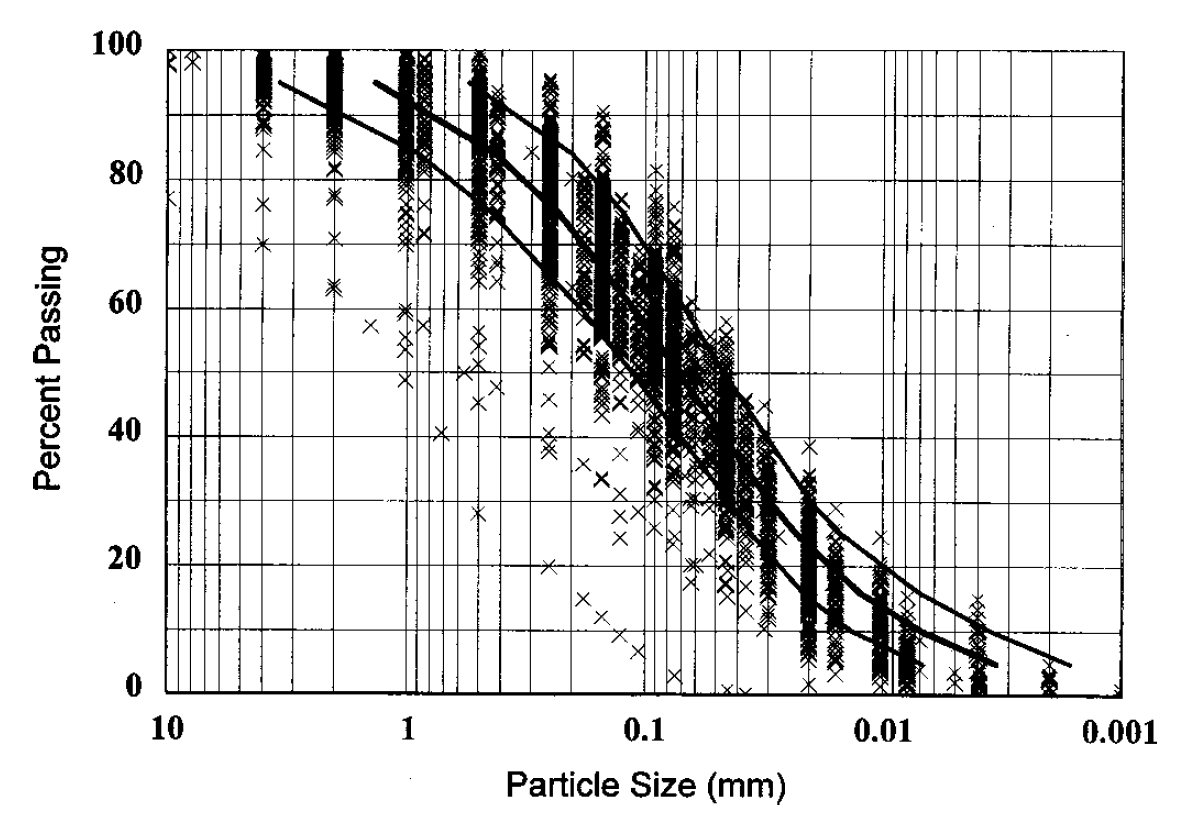
\includegraphics[scale=0.4]{../LaTeX_Report/Carrier2003_Fig1_particle-size-distribution.PNG}
	\caption{Geotechnical particle size distribution: middle curve showing the average distribution; left-hand and right-hand curves showing $\pm$1 standard deviation \citep{carrier2003particle}.}\label{fig:Carrier2003_Fig1_particle-size-distribution}
\end{figure}

In order to parameterize the CDF from Figure \ref{fig:Carrier2003_Fig1_particle-size-distribution}, we make a fit to the model equation
\begin{equation}\label{eq:particle-CDF}
C_{moon} = 1 - \exp\left(\frac{-1}{ax^b+cx^d}\right),
\end{equation}
which is an exponential distribution with two scales defined by $a$ and $c$, with $x$ in units of mm. In \textsf{SciDAVis}, we make the fit with the x-axis on a logarithmic scale to give equal weight to both small and large scaled particles. The results for the curve fit are shown in Figure \ref{fig:Fit-to-CDF}. We found that a simple exponential distribution with a single scale was insufficient, hence the reason we opted for a two-scaled exponential distribution.

\begin{figure}[h!]
	\centering
	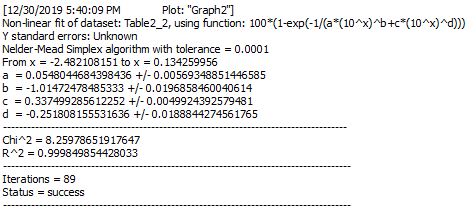
\includegraphics[scale=1]{../LaTeX_Report/Fit-to-CDF.PNG}
	\caption{Non-linear fit of Figure \ref{fig:Carrier2003_Fig1_particle-size-distribution} (the average distribution) with Eq.\ \ref{eq:particle-CDF} in \textsf{SciDAVis}, giving the constants for $a$, $b$, $c$, and $d$.}\label{fig:Fit-to-CDF}
\end{figure}

To compute the probability distribution function (PDF), we can simply take the derivative of the CDF with respect to $x$, which results in the following equation:
\begin{equation}
P_{moon} = -A\frac{abx^{b-1}+cdx^{d-1}}{(ax^b+cx^d)^2}\exp\left(\frac{-1}{ax^b+cx^d}\right),
\end{equation}
where $A$ is the normalization constant. In theory, this should be equal to 1, but since we are not taking our particle size from 0 to infinity, we need to compute the value of $A$. If we assume the particle size can range from $0.001$ mm to $10$ mm, then $A = 1.02218$.
%
%Since our goal is to compute the particle flux mass spectrum, we need to \textit{count} the number of particles from the PDF that make up the mass of $M$ from Eq.\ \ref{eq:HH11_mass-ejected1}. We first need to know the total volume per complete PDF, which is given by
%\begin{equation}\label{eq:VPmoon}
%V_{P_{moon}}(x_{min}) = \frac{4}{3}\pi \int_{x_{min}}^{x_{max}}dx x^3 P_{moon}(x),
%\end{equation}
%where $x_{min} = 0.001$ mm and $x_{max} = 10$ mm. An exact analytic solution of Eq.\ \ref{eq:VPmoon} is quite difficult, but we notice that the integrand $x^3 P_{moon}(x)$ very closely resembles a linear equation within the desired range, see Figure \ref{fig:Fit-to-x3PDF}.
%
%\begin{figure}[h!]
%	\centering
%	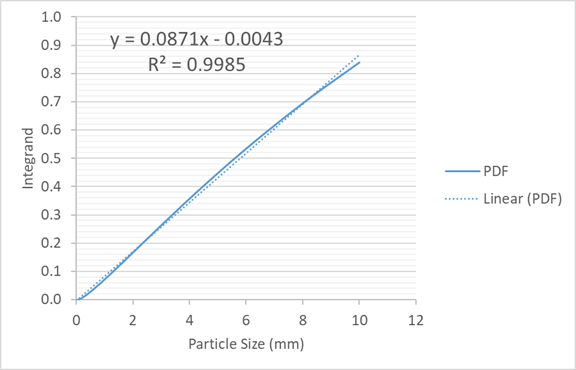
\includegraphics[scale=0.7]{../LaTeX_Report/Fit-to-x3PDF.png}
%	\caption{Linear fit to the integrand $x^3 P_{moon}(x)$.}\label{fig:Fit-to-x3PDF}
%\end{figure}
%
%Therefore, we make the approximation
%\begin{equation}
%x^3 P_{moon}(x) \sim p_0 x + p_1,
%\end{equation}
%where $p_0 = 1/11.48$ and $p_1 = 1/232.6$. The total volume of particles with mass greater than $m_{0} = \frac{4}{3}\pi\rho x_{0}^3$ is given by
%\begin{equation}\label{eq:VPmoon2}
%V_{P_{moon}}(x_{0}) = \frac{4}{3}\pi \left[\frac{1}{22.96}\left(x_{max}^2 - x_{0}^2\right) - \frac{1}{232.6}\left(x_{max} - x_{0}\right)\right],
%\end{equation}
%where $V_{P_{moon}}(x_{min}) = 18.06377$ mm$^3$. Given the density of the regolith $\rho$, we can then compute the total mass of the particles from the PDF.



%%%%%%%%%%%%%%%%%%%%%%%%%%%%%%%%%%%%%%%%%%%%%%%%%%%%%%%%%%%%%%%%%%
%%%%%%%%%%%%%%%%%%%%%%%%%%%%%%%%%%%%%%%%%%%%%%%%%%%%%%%%%%%%%%%%%%
\subsection{Ejecta Distance, Speed, and Angle Relations}


We would like to relate the distance from the meteorite impact to the secondary ejecta impact site by the secondary ejecta speed $v$ and angle $\gamma$ from zenith. If we assume the Moon is a perfect sphere with no atmosphere, we can calculate this distance by following the elliptical path the ejecta makes. The semi-major axis and eccentricity of the elliptical orbit are given by\footnote{See Eqs.\ 4.30 and 4.32 from http://www.braeunig.us/space/orbmech.htm.}
\begin{equation}\label{eq:a_of_v}
\frac{a}{r_m} = \frac{1}{2\left(1-\frac{v^2}{v_{esc}^2}\right)},
\end{equation}
where $r_m = 1737.1$ km is the radius of the Moon and $v_{esc} = 2.38$ km/s is the Moon's escape velocity, and
\begin{equation}\label{eq:e_of_v}
e = \sqrt{\left(\frac{2v^2}{v_{esc}^2}-1\right)^2\sin^2\gamma + \cos^2\gamma},
\end{equation}
where we employed the fact that the gravity of the Moon is $g = GM/r_m^2$ and the escape velocity is related by $v_{esc} = \sqrt{2gr_m}$. The third equation we need gives the location in the elliptical orbit by the angle $\beta$ from the perilune, the semi-major axis $a$, and the eccentricity $e$ by
\begin{equation}\label{eq:r_elliptical_orbit}
r = \frac{a(1-e^2)}{1+e\cos\beta}.
\end{equation}
Solving for $\cos\beta$ in Eq.\ \ref{eq:r_elliptical_orbit}, we have
\begin{equation}\label{eq:cos_elliptical_orbit}
\cos\beta = \frac{1}{e}\left(\frac{a(1-e^2)}{r}-1\right).
\end{equation}
In addition, we also need the equation for $\sin\beta$, which is given by (using a right triangle)
\begin{equation}
\sin\beta = \frac{1}{e}\sqrt{e^2-\left[\frac{a(1-e^2)}{r}-1\right]^2},
\end{equation}
so that $\tan\beta$ is
\begin{equation}\label{eq:tan_beta}
\tan\beta = \frac{\sqrt{e^2-\left[\frac{a(1-e^2)}{r}-1\right]^2}}{\frac{a(1-e^2)}{r}-1}.
\end{equation}

We found that the distance the secondary ejecta travels is given by the arc length of Moon the orbit travels greater than the radius of the Moon:
\begin{equation}\label{eq:D}
D = 2(\pi-\beta)r_m,
\end{equation}
or solving for the angle $\beta$,
\begin{equation}
\beta = \pi - \frac{D}{2r_m}.
\end{equation}
Using Eqs.\ \ref{eq:a_of_v} and \ref{eq:e_of_v}, we can write
\begin{equation}
\frac{a}{r_m}(1-e^2) = 2\frac{v^2}{v_{esc}^2}\sin^2\gamma,
\end{equation}
so Eq.\ \ref{eq:tan_beta} becomes \citep[c.f., Eq.\ (1) of][]{vickery1986size}
\begin{equation}\label{eq:ejecta_distance}
\tan\left(\frac{D}{2r_m}\right) = \frac{2\frac{v^2}{v_{esc}^2}\sin\gamma\cos\gamma}{1-2\frac{v^2}{v_{esc}^2}\sin^2\gamma} = \frac{\frac{v^2}{v_{esc}^2}\sin(2\gamma)}{\frac{v^2}{v_{esc}^2}[\cos(2\gamma)-1]+1}
=\frac{2\frac{v^2}{v_{esc}^2}\tan\gamma}{1+(1-2\frac{v^2}{v_{esc}^2})\tan^2\gamma}.
\end{equation}




%Therefore, we insert Eqs.\ \ref{eq:a_of_v}, \ref{eq:e_of_v}, and \ref{eq:D} into Eq.\ \ref{eq:cos_elliptical_orbit}, so that we now have the distance as a function of ejecta speed and angle from the zenith
%\begin{equation}\label{eq:ejecta_distance}
%\cos\left(\frac{D}{2r_m}\right) = \frac{1 - \frac{2v^2}{v_{esc}^2}\sin^2\gamma}{\sqrt{\left(1-\frac{2v^2}{v_{esc}^2}\right)^2\sin^2\gamma + \cos^2\gamma}}.
%\end{equation}
%Solving for the ejecta speed $v$, we can rewrite Eq.\ \ref{eq:ejecta_distance} in terms of the ejecta distance $D$ and zenith angle $\gamma$
%\begin{equation}
%\frac{v^2}{v_{esc}^2} = \frac{1}{2}\frac{\sin^2\left(\frac{D}{2r_m}\right)}{\cos^2\left(\frac{D}{2r_m}\right) - \sin^2\gamma}\left[\cot\left(\frac{D}{2r_m}\right)\cot\gamma - 1\right].
%\end{equation}
% Run plotSpeedAngleDistance.py
\begin{figure}[h!]
	\centering
	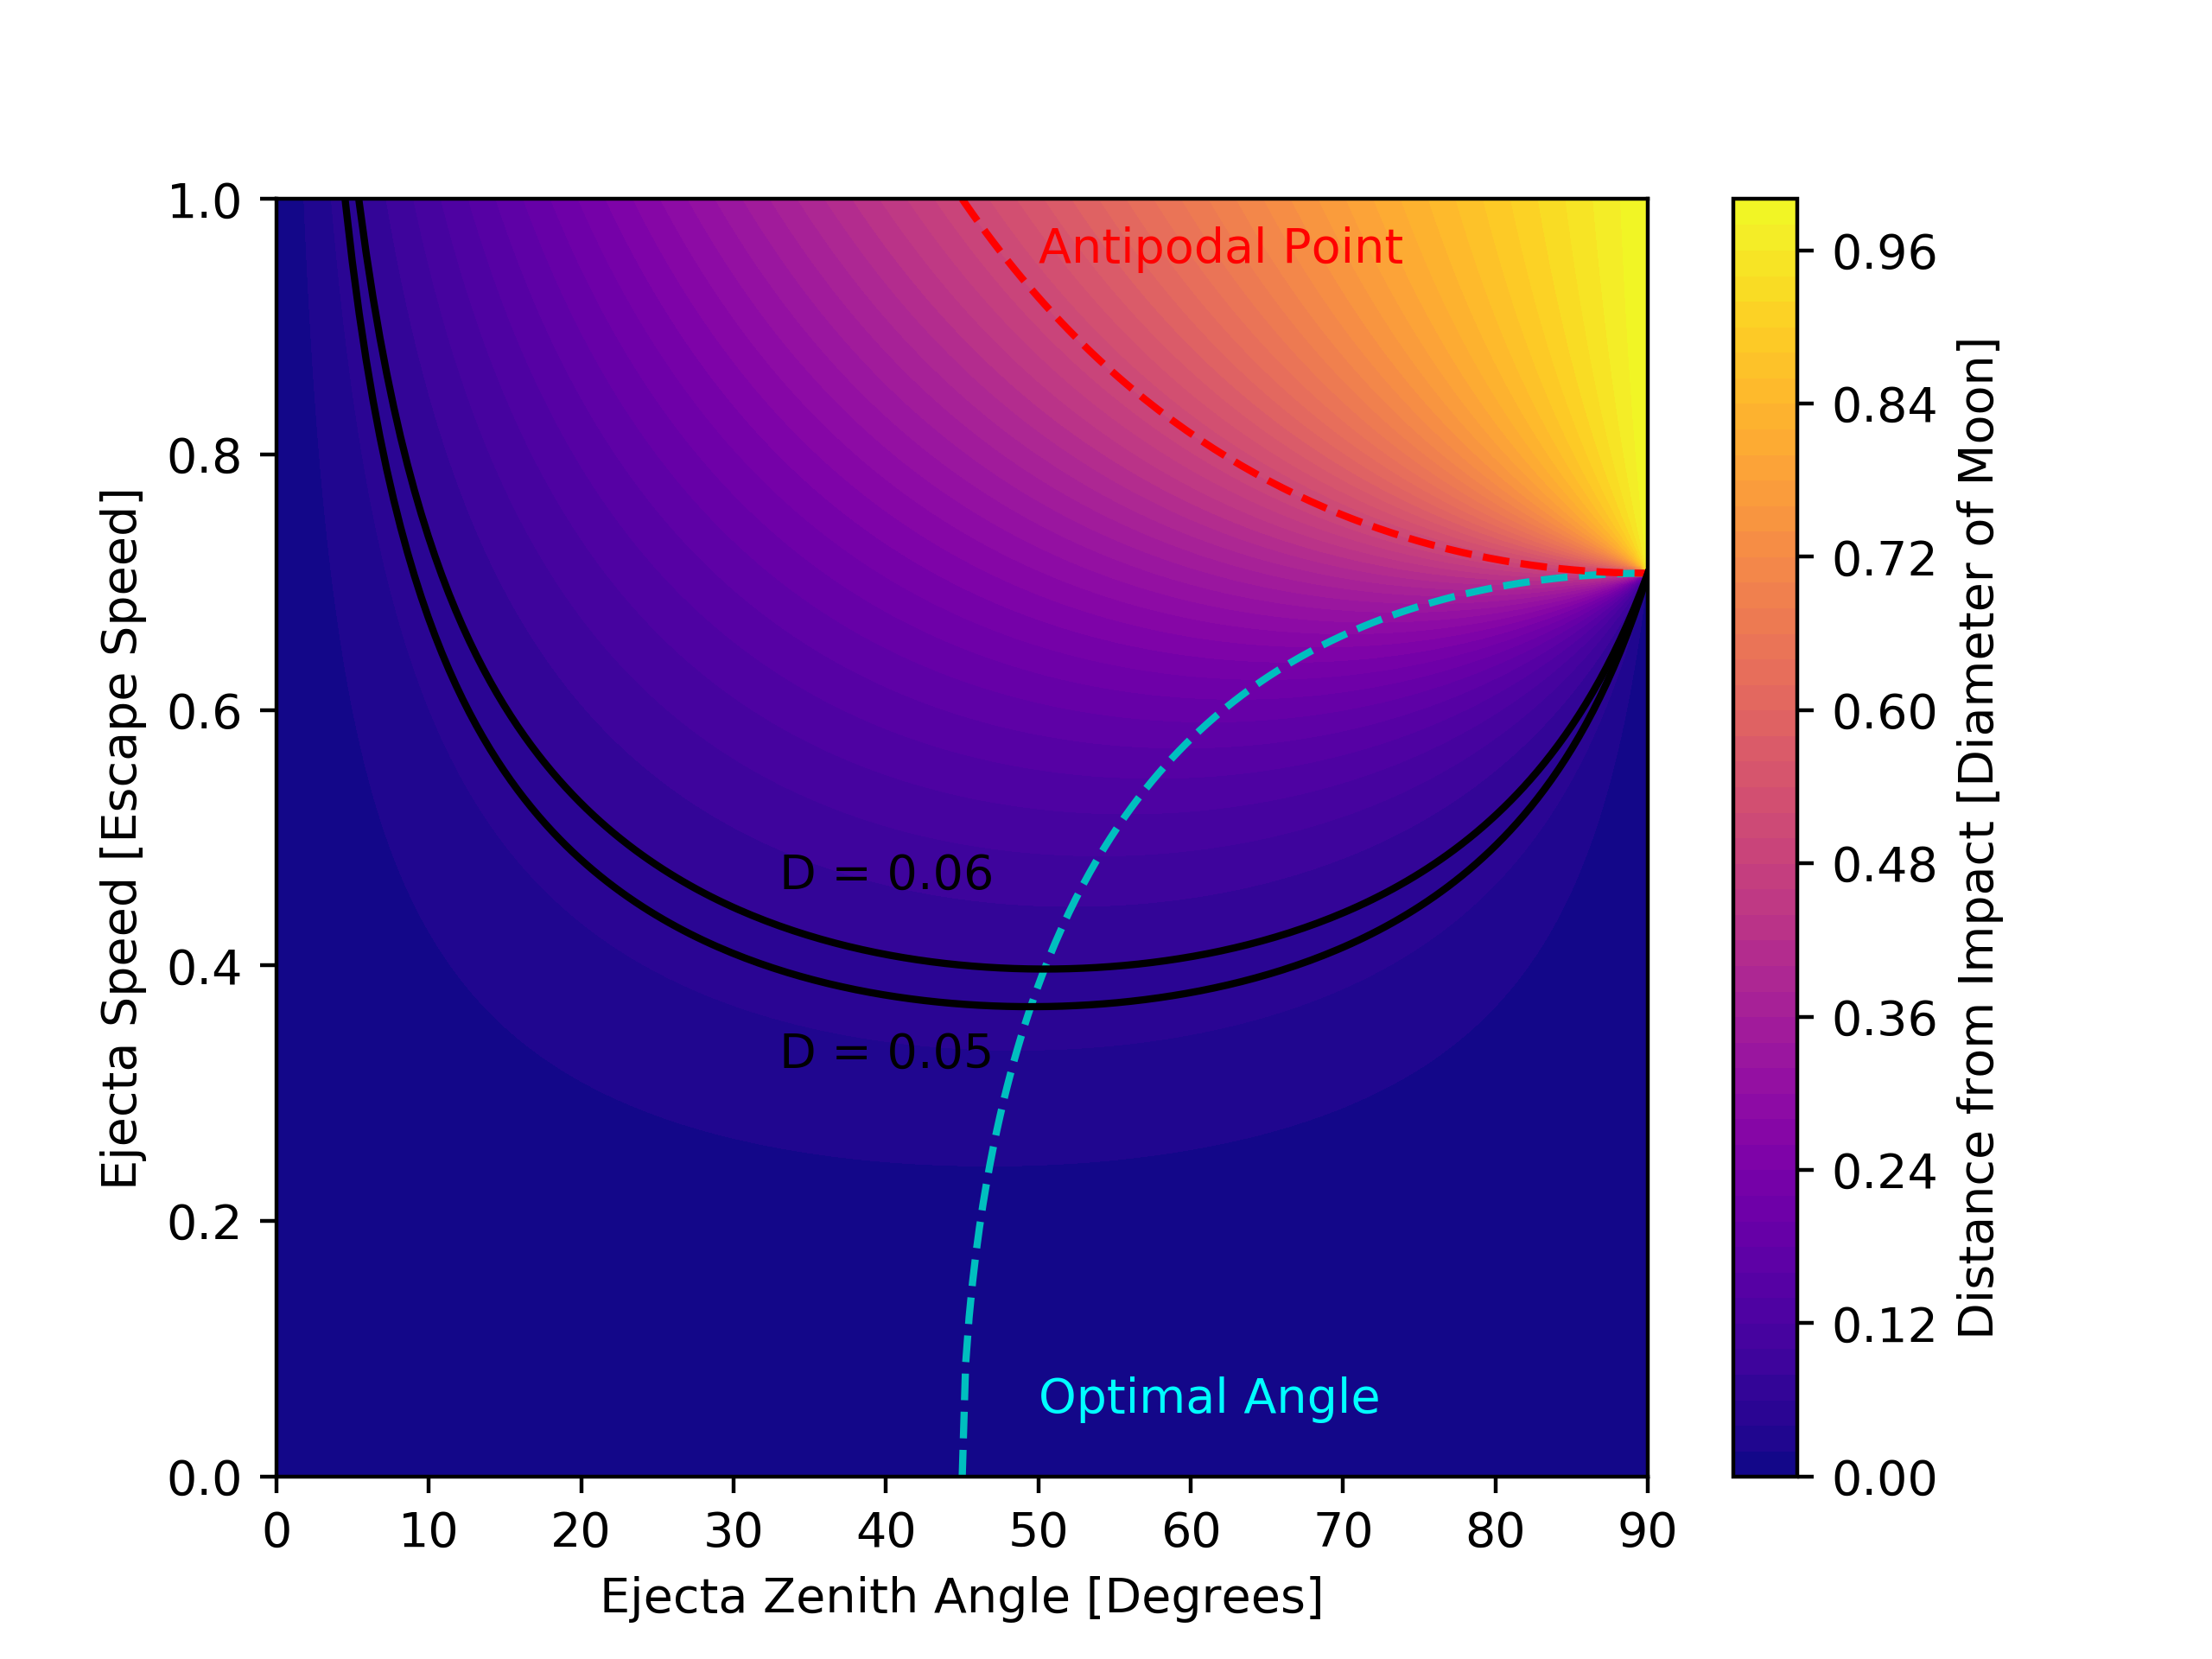
\includegraphics[scale=0.85]{../LaTeX_Report/Distance_vs_EjectaSpeed_and_ZenithAngle.png}
	\caption{The color gradient shows the distance a projectile goes with a given ejected speed and zenith angle. The cyan dashed line gives the optimal angle for a given speed to reach the furthest distance, i.e., Eq.\ \eqref{eq:opt_angle}. The red dashed line shows for which pairs of speeds and zenith angles are required to hit the antipodal point. As an example, all ejecta with speed and angle pairs between the two black curves will reach a location between 0.05 and 0.06 lunar circumference units away, using Eq.~\eqref{eq:speed_asof_distance_angle}.}\label{fig:Distance_vs_EjectaSpeed_and_ZenithAngle}
\end{figure}



For $D \ll 2r_m$, the optimum angle that gives the smallest velocity needed is $45^\circ$. In other words, for a given velocity, the greatest distance is found by taking $\gamma = 45^\circ$. However, if the distance $D$ is roughly the same order as the diameter of the Moon $2r_m$, ($D > 0.01\times 2r_m$), then the optimal angle from zenith is greater than $45^\circ$, i.e.\ a shallower angle to the horizon. This is because at large velocities, the curvature of the Moon comes into play. For larger velocities, there are also angles $\gamma$ that cannot reach a distance $D$. Allowable angles (in radians) that can travel a distance $D$ are defined by
\begin{equation}
\gamma > \frac{D}{4r_m}.
\end{equation}
In other words, the maximum distance the ejecta can reach for a given angle is
\begin{equation}
D = 4\gamma r_m.
\end{equation}
For example, from this equation we can conclude that for $\gamma < 45^\circ$, the ejecta will not reach the antipodal point, see Figure \ref{fig:Distance_vs_EjectaSpeed_and_ZenithAngle}.


Solving for $v$ we have
%\begin{equation}
%\frac{v^2}{v_{esc}^2} = \left[1-\cos(2\gamma)+\sin(2\gamma)\cot\left(\frac{D}{2r_m}\right)\right]^{-1}
%\end{equation}
\begin{equation}\label{eq:speed_asof_distance_angle}
\frac{v}{v_{esc}} = \frac{+1}{\sqrt{\sin(2\gamma)\left(\cot\left(\frac{D}{2r_m}\right)+\tan\gamma\right)}}
= \frac{+1}{\sqrt{1+\sin(2\gamma)\cot\left(\frac{D}{2r_m}\right)-\cos(2\gamma)}}.
\end{equation}
We can also solve for the zenith angle $\gamma$, given by
\begin{equation}\label{eq:gammaVs_V_D}
\cot\gamma = x^2\cot\left(\frac{D}{2r_m}\right) \pm \sqrt{x^4\cot^2\left(\frac{D}{2r_m}\right) + (2x^2-1)},
\end{equation}
where $x = v/v_{esc}$. Solving for the discriminant, the minimum $x$ can be for a given distance $D$ is
\begin{equation}
x_{min}^2 = \tan^2\left(\frac{D}{2r_m}\right)\left[\csc\left(\frac{D}{2r_m}\right)-1\right].
\end{equation}
Plugging into Equation \ref{eq:gammaVs_V_D}, the optimal angle from zenith is given by
\begin{equation}\label{eq:opt_angle}
\cot\gamma_{opt} = \sec\left(\frac{D}{2r_m}\right) - \tan\left(\frac{D}{2r_m}\right).
\end{equation}
In terms of $x$, we have
\begin{equation}
\cos(2\gamma_{opt}) = \frac{x^2}{x^2-1}.
\end{equation}
Once $D > \pi r_m$, the optimal angle is $\gamma = 90^\circ$, i.e., parallel to the horizon. For small distances $D \ll 2r_m$, the optimal angle is $\gamma = 45^\circ$, as mentioned above.


%%%%%%%%%%%%%%%%%%%%%%%%%%%%%%%%%%%%%%%%%%%%%%%%%%%%%%%%%%%%%%%%%%
%%%%%%%%%%%%%%%%%%%%%%%%%%%%%%%%%%%%%%%%%%%%%%%%%%%%%%%%%%%%%%%%%%
\subsection{Distance and Bearing}\label{ssec:Distance_and_Bearing}
% see https://www.movable-type.co.uk/scripts/latlong.html

Given two latitude-longitude points on a sphere, $(\phi_1, \theta_1)$ and $(\phi_2, \theta_2)$, we can compute the distance and bearing following Chris Veness's webpage\footnote{\url{https://www.movable-type.co.uk/scripts/latlong.html}}.

The distance D is given by the equation
\begin{equation}\label{eq:shortdistance-between-latlon-points}
\tan\left(\frac{D}{2r_m}\right) = \sqrt{\frac{a}{1-a}},
\end{equation}
where $a$ is given by
\begin{equation}
a = \sin^2(\Delta\phi/2) + \cos\phi_1\cos\phi_2\sin^2(\Delta\lambda/2),
\end{equation}
for $\Delta\phi = \phi_2-\phi1$ and $\Delta\lambda = \lambda_2-\lambda_1$. Solving for the distance and simplifying, we have
\begin{equation}
D = 2r_m\arcsin(\sqrt{a}),
\end{equation}
or
\begin{equation}
D = 2r_m\arccos(\sqrt{1-a}).
\end{equation}

Other useful expressions involving trigonometric functions of $D/r_m$ are
\begin{align}
\sin(D/r_m) &= 2\sqrt{a(1-a)},\\
\cos(D/r_m) &= 1-2a,\\
\tan(D/r_m) &= \frac{2\sqrt{a(1-a)}}{1-2a}.
\end{align}

Eq.\ \eqref{eq:shortdistance-between-latlon-points} is the shortest distance between two coordinate points. For the long-distance, use
\begin{equation}
\tan\left(\pi-\frac{D}{2r_m}\right) = -\tan\left(\frac{D}{2r_m}\right) = \sqrt{\frac{a}{1-a}}.
\end{equation}

The initial bearing $\theta$ (from due East) is given by the following equation (assuming the short-distance):
\begin{equation}\label{eq:initial-bearing-shortdist}
\tan\theta_{i(1,2)} = \frac{\sin\Delta\lambda\cos\phi_2}{\cos\phi_1\sin\phi_2-\sin\phi_1\cos\phi_2\cos\Delta\lambda}.
\end{equation}
To find the final bearing (assuming the short-distance), swap $\phi_1\longleftrightarrow\phi_2$ and $\lambda_1\longleftrightarrow\lambda_2$ and reverse the angle such that
\begin{equation}\label{eq:final-bearing-shortdist}
\theta_{f(1,2)} = (\theta_{i(2,1)} + \pi)\mod 2\pi.
\end{equation}

In order to compute the initial and final bearing for the long-distance trajectory, add $\pi$ and then mod by $2\pi$ to Eqs.\ \eqref{eq:initial-bearing-shortdist} and \eqref{eq:final-bearing-shortdist}. In other words, swap initial and final bearings $\theta_{i(1,2)}\longleftrightarrow\theta_{f(1,2)}$.\\

We can also get the final latitude and longitude if we are given the distance $D$ and bearing $\theta$ from the starting location. The latitude and longitude are given by
\begin{align}
\phi_2 &= \arcsin\left[\sin\phi_1\cos(D/r_m) + \cos\phi_1\sin(D/r_m)\cos\theta\right], \\
\lambda_2 &= \lambda_1 + \arctan\left[\frac{\sin\theta\sin(D/r_m)\cos\phi_1}{\cos(D/r_m) - \sin\phi_1\sin\phi_2}\right].
\end{align}

%%%%%%%%%%%%%%%%%%%%%%%%%%%%%%%%%%%%%%%%%%%%%%%%%%%%%%%%%%%%%%%%%%
%%%%%%%%%%%%%%%%%%%%%%%%%%%%%%%%%%%%%%%%%%%%%%%%%%%%%%%%%%%%%%%%%%
%\section{References}
\cleardoublepage
\phantomsection
\addcontentsline{toc}{section}{References}
\bibliographystyle{agu}
\bibliography{../LaTeX_Report/report}

\end{document}